\documentclass[12pt, a4paper]{report} \usepackage[titletoc]{appendix}
%\linespread{1.5}
%\usepackage{lineno}
%\linenumbers
\usepackage{multirow}
\usepackage{hhline}
\usepackage{array}
\usepackage{caption}
\usepackage{subcaption}
\usepackage{float}
\usepackage{graphicx}
	\graphicspath{{images/}} 
\usepackage{geometry}
	\geometry{a4paper,left=3cm,top=3cm,bottom=3cm,right=3cm}
\usepackage{array}
\usepackage{multirow}
\usepackage{hyperref}
	\hypersetup{colorlinks=true,allcolors=blue}
\usepackage{hypcap}
\usepackage[linesnumbered,ruled]{algorithm2e}
\usepackage{courier}
\usepackage{listings}
\lstset{
	basicstyle=\ttfamily,
	frame=none, 
	breaklines=true,
	numbers=left,
	xleftmargin=2.5em,
	framexleftmargin=0em,
	emphstyle=\textbf,
	float=t
}
\lstdefinestyle{ocl}{
	emph={
		context, inv
	}
}
\lstdefinestyle{cbp}{
	basicstyle=\ttfamily\scriptsize,
	emph={
		session, create, of, type,
		set, to, add, hire
	}
}
\lstdefinestyle{xmi}{
	basicstyle=\ttfamily\scriptsize,
	emph={
		Node, children,
		Employee, manages
	}
}
\lstdefinestyle{xml}{
	basicstyle=\ttfamily\scriptsize,
	emph={
		register, create, add, to, resource,
		from, eattribute, remove, ereference,
		set, unset, session, Roy, Jen,
		Moss, Richmond
	}
}
\lstdefinestyle{java}{
	basicstyle=\ttfamily\scriptsize,
	emph={
		case, UNSET,
		instanceof, else, if, void,
		new, UnsetEAttributeEvent,
		UnsetEReferenceEvent,
		@override, public, class, extends
	}
}
\lstdefinestyle{eol}{
	basicstyle=\ttfamily\scriptsize,
	emph={
		var, new, for, in, create, set, of, with, 
		unset, to, add, remove, delete, register,
		from, position, from, move-within, session, \.
	}
}

\setlength{\parindent}{1cm}
\setlength{\parskip}{0.1cm}


\begin{document}

\begin{titlepage}
 \begin{center}

\textbf{Progress Report}
\vspace{1cm}

\textbf{\large Model Change-Detection, Comparison, and Merging\\using Change-Based Persistence}
\vspace{1cm}

Alfa Ryano Yohannis\\
ary506@york.ac.uk
\vspace{1cm}

Supervisors:\\
Dimitris Kolovos\\
Fiona Polack\\
\vspace{1cm}

Department of Computer Science\\
University of York\\
United Kingdom\\
\vspace{1cm}
\today
 
\vfill
 
\end{center}
\end{titlepage}


\begin{abstract}
\addcontentsline{toc}{chapter}{Abstract}
Most of the models in Model-Driven Engineering are persisted in state-based formats. As an alternative, change-based persistence (CBP) also has been proposed. State-based persistence (SBP) offers faster model loading time than change-based representation but outperformed by its counterpart when it comes to persisting and detecting changes of models. This research aims to integrate both types of persistence to produce a hybrid model persistence to gain the advantages of both approaches. The main impact of CBP on faster persisting and detecting changes, its knock-on effects on the model comparison and merging, as well as efforts to reduce its side effects will be investigated and evaluated. So far, an initial implementation has been developed, and an algorithm to reduce the loading time of CBP models has been proposed. Based on this work's previous investigation, change-based approach persists changes of models faster than its state-based counterpart, and the proposed algorithm has successfully loaded CBP models faster than loading the models naively. The initial implementation has been presented in a workshop, and the proposed algorithm has been submitted to a conference and currently under review. A research plan to complete this work in the next two years is also explained in this report.
\end{abstract}

\tableofcontents
\addcontentsline{toc}{chapter}{Contents}

\listoffigures
\newpage
 
\listoftables
\newpage

\lstlistoflistings
\newpage

\chapter{Introduction}
\label{ch:introduction}
This Chapter briefly presents the background of this work as well as the research questions that will addressed in this work. Several research objectives are then defined to answer the research questions. Research outputs and scoping are also presented. 

\section{Background}
\label{sec:background}
Existing approaches for file-based model persistence in metamodelling architectures such as MOF and EMF are predominately state-based. In such approaches, model files contain snapshots of the models' contents, and activities like version control and change detection are left to external systems such as file-based version-control systems and model differencing facilities. Activities such as change-detection -- to find parts that already changed of a model compared to its previous version/ancestor -- and model comparison -- to find the differences between models that come from the same ancestor -- are computationally consuming for state-based models. As a result,  the expensive cost can diminish the performance benefits of incremental execution of model management programs when working with large models, and it can become a burden when large models are developed in a collaborative setting.

In contrast to persisting the \emph{state} of models, a change-based approach persists the full sequence of \emph{changes} made to models instead. The change-based approach comes with a number of envisioned benefits over state-based persistence, such as the ability to detect changes much faster and more precise, which can then have positive knock-on effects on helping developers compare and merge models in collaborative modelling environments, as well as on facilitating faster incremental model validation and transformation \cite{rath2012derived,ogunyomi2015property}. Change-based approach is faster in change-detection since changes of a model are already persisted in ordered manner based on the sequence of their occurrence and therefore they only need to be identified sequentially without having to explore all elements of the model and compare them to the elements of its previous model. Change-based approach is more precise since the changes are persisted with finer-granularity informations (e.g. the order of the changes, previous values, etc.). Nevertheless, change-based persistence comes at the cost of larger and ever-growing model files, and increased model loading time since all recorded changes need to be replayed to reconstruct a model's state \cite{yohannis2017turning}.

The expensive cost of state-based models in change-detection and model differencing motivates this work to investigate change-based persistence to enable fast model comparison and differencing, and scales for large models developed in a collaborative setting. So far, this research had already attempted to reduce the loading time of change-based persistence (CBP) models and can save up 44\% loading time compared to loading CBP models naively (see Subsection \ref{sec:load_time_reduction_of_change-based_models} and Chapter \ref{ch:research_plan}, Task 1). However, since the optimised loading time is still significantly longer than the loading time of state-based persistence (SBP), this research propose a hybrid model persistence (HMP) that is persistence using change-based and state-based approaches side-by-side. Every event of model modification is persisted into a change-based representation and the change is applied to a state-based representation simultaneously. This dual persistence enables faster change-detection while still maintains the loading time of state-based persistence and its other advantages as well, such as partial and lazy loading of model elements \cite{ran2016partial,daniel2016neoemf}.  

\section{Research Questions}
\label{sec:research_questions}
This work aims to introduce change-based persistence, as an alternative approach to state-based persistence, to persist models for faster change-detection, and use it side-by-side with state-based persistence to produce a hybrid model persistence to gain the benefits of both persistence approaches. The faster change-detection, knock-on effects on model comparison and merging, and efforts to reduce its increasing file size and loading time will also be investigated. Thus, this work aims to answer these following research questions: 
\begin{enumerate} 
	\item \textbf{How to implement CBP to models?} 
	
	The concept of change-based persistence has to be translated into an implementation in a modelling framework context so that it can be applied for model persistence, and therefore its impact on model change-detection, model comparison, and model merging can be assessed. It is expected that every changes made to a model can be persisted by the implementation and can produce the same model as persisted in state-based format after loading.
	
	\item \textbf{How to reduce the increasing file size and loading time of CBP models? And to what extent can they be reduced?} 
	
	CBP comes with downsides on larger, increasing file size and loading time. Mitigating these side effects will optimise the use of CBP. It is expected that the mitigation approaches can produce loading time that is negligible to the loading time of state based format and significantly faster than loading CBP models naively, and significantly reduce file size compared to the naive approach of saving CBP files. 
	
	\item \textbf{How to use CBP and SBP side-by-side for model persistence? And to what extent is its impact on saving time, disk space usage, loading time, and change-detection?} 
	
	Since reducing the loading time of CBP had been attempted and the optimised loading time is still significantly longer than SBP's loading time, this research will try to use both persistence side-by-side so that the fast change-detection of CBP and the fast loading time of SBP can still be obtained simultaneously. 
	
	The impact of this hybrid approach on several qualities will also be investigated. It is expected that: (1) HMP models will be significantly slower than CBP models on persisting changes and slightly slower than SBP models on saving time as HMP needs to save changes to both types of persistence. (2) HMP consumes more disk space compared to CBP or SBP alone since HMP use two types of persistence simultaneously. (3) HMP models has loading time that is negligible to the loading time of SBP models since only the state-based part of HMP that is active for loading models. (4) HMP models has negligible change-detection time compared to CBP models since only the change-based part of HMP that is active for detecting changes.        
	
	\item \textbf{How to compare change-based models that come from the same ancestor? And how does the comparison of change-based models perform compared to state-based model comparison?} 
	
	The knock-on effect of faster change-detection on model comparison will also be investigated. Due to the nature of change-based models, the mechanism to perform change-based model comparison will differ substantially from current state-based model comparison. It is expected that comparison of CBP models will be significantly faster than the comparison of SBP models.   
	
	\item \textbf{How to merge different change-based models that come from the same ancestor? And how does the merging perform compared to model merging in state-based persistence?}
	
	Another knock-on effect of faster change-detection of CBP is faster model merging. Similar to CBP model comparison, the mechanism to merge CBP models will differ substantially from merging SBP models. It is expected that the CBP model merging will be much faster than SBP model merging.   
	
\end{enumerate}

\section{Research Objectives}
\label{sec:research_objectives}
This research aims to meet the following research objectives to answer the research questions.
\begin{enumerate}
	\item Develop an implementation of CBP so it can be applied to persist models in change-based format, and evaluate the correctness of change-based models that it produces. 
	\item Propose approaches (i.e. compression algorithm, binary format, or the use of graph database) to reduce file size and loading time of change-based persistence models, and evaluate its performance against the naive approach. 
	\item Develop an implementation of hybrid model persistence so that change-based and state-based approach can be used side-by-side to persist models, and evaluate its impact on saving time, disk space usage, loading time, and change-detection.
	\item Develop an algorithm to compare the change-based part of hybrid persistence models, and evaluate its execution time and memory footprint against model comparison in state-based only.
	\item Develop an algorithm to merge different hybrid persistence models, and evaluate its execution time and memory footprints against model-merging in state-based only. 
\end{enumerate}

\section{Research Outputs}
\label{sec:research_outputs}
By the end of this research, these following outputs will have been produced:
\begin{enumerate}
	\item A prototype for hybrid model persistence and change-based persistence. The implementation of change-based persistence precedes the implementation of hybrid model persistence and will be used as a component in the latter persistence along with existing state-based persistence. 
	\item Algorithms -- including their implementation and evaluation -- for file size and loading time reduction, change-detection (finding parts that already changed of a model compared to its previous version/ancestor), model comparison (finding differences between models that come from the same ancestor), and model merging of change-based persistence.
	\item A publication for each research question, and a thesis report of this research. 
\end{enumerate}


\section{Research Scoping}
\label{sec:research_scoping}
This research plan to use change-based and state-based persistence side-by-side to persist models. Moreover, since there are several existing instances of state-based persistence, XMI and NeoEMF \cite{daniel2016neoemf} has been chosen for this research. The former is a standard model persistence format, and the latter is a recent work that leverages the use of NoSQL databases for large-scale model persistence. XMI was already used as a baseline in the Task 1 (see Chapter \ref{ch:evaluation_strategy}) that has been completed for measuring the performance of the proposed algorithm in reducing the loading time of CBP models. For the other incoming tasks, NeoEMF will be used as the representation of state-based persistence.

\chapter{Research Plan}
\label{ch:research_plan}
For the next two years, this research plans to execute these following tasks. In every task, the correctness, performance, advantages, and shortcomings of the proposed change-based approaches are compared to equivalent approaches in state-based persistence. Every task, except Thesis Writing-Up, is expected to produce a publishable paper. The research timetable is displayed in Table \ref{table:research_timetable}.

\begin{table}[h]
	\centering
	\caption{Change-Based Persistence Research timetable.}
	\label{table:research_timetable}
	\begin{tabular}
		{|>{\centering\arraybackslash}p{1.1cm}|>{\centering\arraybackslash}p{4cm}|>{\centering\arraybackslash}p{4cm}|>{\centering\arraybackslash}p{4cm}|}
		\hline 
		Month & 2017 & 2018 & 2019 \\ 
		\hline 
		1               & \multirow{6}{4cm} & \multirow{3}{4cm}{\centering Hybrid Model Persistence}  & \multirow{2}{4cm}{\centering Task 5: File Size Reduction} \\ 
		\hhline{-~~~}2  & & &  \\ 
		\hhline{-~~-}3  & & & \textbf{40-Minute Seminar} \\ 
		\hhline{-~--}4  & & \textbf{Thesis Outline} & \multirow{5}{4cm}{\centering Task 6: Thesis Writing-Up}  \\ 
		\hhline{-~-~}5  & & \multirow{3}{4cm}{\centering Task 3: Model Comparison} & \\ 
		\hhline{-~~~}6  & & & \\ 
		\hhline{--~~}7  & \multirow{4}{4cm}{\centering Task 1: Change-Based Persitence \& Loading Optimisation} & &  \\  
		\hhline{-~-~}8  & & \textbf{Thesis Audit}  &  \\ 
		\hhline{-~--}9  & & \multirow{4}{4cm}{\centering Task 4: Model Merging} & \textbf{Thesis Submission} \\  
		\hhline{-~~-}10 & &  &  \\ 
		\hhline{--~~}11 & \textbf{Progress Report} &  &  \\ 
		\hhline{--~~}12 & \multirow{1}{4cm}{\centering Task 2:} & &  \\ 
		\hline 
	\end{tabular} 
\end{table}

\begin{itemize}
	\item \textbf{Task 1: Change-Based Persistence \& Loading Optimisation.}  The aim of this task is to prepare the ground for this research by developing a language-independent change-based model persistence format that can be used as a basis for hybrid model persistence, change-detection, model comparison, and model merging. Also, this task aims to design and implement an optimisation algorithm that reduces the loading time of change-based models by cancelling out events superseded by subsequent events. Five months was allocated for this task and it already finished. Two papers had been written in this task. One paper was presented in a workshop and another paper is under review.
	\item \textbf{Task 2: Hybrid Model Persistence.} It is conceivable that in some cases, persisting the entire change history in a model file will be an overkill and that persisting a base state and editing sessions operating on that state (e.g. capturing ``recent" changes) will be preferable. This task will extend state-based format so that it can incorporate information of changes. It will also investigate how integration with version control systems such as Git can enable the reconstruction of the full change history of a model in a transparent way. Four months will be allocated for this task. 
	\item \textbf{Task 3: Model Comparison.} This task will design and implement efficient algorithms for comparing change-based models, with a focus on models with shared editing histories. Due to the nature of change-based models, it is expected that the comparison algorithms developed in this task will differ substantially from current state-based model comparison algorithms. Three months will be allocated for this task. 
	\item \textbf{Task 4: Model Merging.} In this task, the candidate will design and implement algorithms for conflict resolution and merging of change-based models. The algorithms developed in this task will leverage/extend the comparison algorithms developed in Task 3. Four months will be allocated for this task. 
	\item \textbf{Task 5: File Size Reduction.} This task will design and implement compression algorithms that can eliminate redundant changes within and across editing sessions, in order to reduce the storage requirements for persisting change-based models (e.g. if the value of a single-valued model element attribute is modified more than once in the context of an editing session, only the last modification event can be persisted). Since an algorithm had already been applied to reduce the loading time of change-based files, a similar algorithm can be applied to reduce the size of change-based files. Thus, only two months will be allocated for this task. It is important to notice that since the contribution of this task is relatively not as significant as other tasks, it is given a lower priority than any other task and preferably to be dropped regarding limited time available.
	\item \textbf{Task 6: Thesis Writing-Up.} Four months will be allocated for the write-up of the doctoral thesis.  
\end{itemize}

\chapter{Evaluation Strategy}
\label{ch:evaluation_strategy}
 For the evaluation where there are existing approaches that the algorithms and tools developed in this research seek to outperform (e.g. change-based incremental validation vs. state-based incremental validation), comparative evaluation will be conducted to assess the benefits and limitations of the approaches. For algorithms and tools that have no direct competitors in the literature, such as reducing file size and loading time of change-based models, their contributions will be assessed in comparison to the baseline they seek to improve (e.g. in this case, persisting and replaying full change histories).  

This research is divided into several tasks (see Chapter \ref{ch:research_plan}) with each task addresses a different problem. The evaluation strategy for each task is as follows. 
\begin{enumerate}
	\item \textbf{Task 1: Change-Based Persistence \& Loading Optimisation.} In this task, the implementation of change-based persistence is evaluated for its correctness by comparing the eventual state of a loaded CBP model to its state-based persistence in XMI. If they are equal, it means that the implementation has successfully loaded the change-based model. This comparison is performed across models with different size and metamodels.    
    
    The proposed algorithm to optimise the loading of CBP models was evaluated against the naive loading of CBP models and the loading of XMI models on loading times and memory footprints. Moreover, this research also compares the optimised CBP models against the naive CBP and XMI models on the time required to save changes made on them. For the evaluation, synthetic models of different sizes were used. The evaluation for this task had been completed, and the results are presented in Subsection \ref{subsec:performance_evaluation}.
	
	Given that CBP is a very recent contribution, and it is almost impossible to find any existing datasets containing real-world models expressed in a change-based format, this research uses synthetic models for experiments. Nevertheless, instead of synthesising the models arbitrarily as had been performed in the Task 1, the CBP models will be reverse engineered from several projects hosted in version controls (e.g. GitHub, SVN). The differences between each version are translated into change events in CBP models. Therefore, the generated CBP models are more representative since they are generated from real-world projects. This strategy will be applied in the subsequent tasks.
	
	\item \textbf{Task 2: Hybrid Model Persistence (HMP).} Evaluation is performed to gain understanding the effects of HBP, using CBP and SBP side-by-side to persist models, on saving changes, disk space usage,change-detection, and loading/query time. HMP will be compared against CBP on the time required to save changes and the disk space usage. The saving time and the disk space usage are selected as the dimensions of measurement since HMP requires model changes to be persisted into two kinds of persistence -- CBP and SBP -- which means it requires more saving time and disk space usage. HMP will also be compared against SBP on the time used for change-detection and loading/queries since the intention of using CBP and SBP side-by-side is to gain faster change-detection while maintaining the loading/query time of SBP. The comparison will be performed across different model datasets that are vary in size and metamodel.
	
	\item \textbf{Task 3: Model Comparison.} Evaluation is performed to gain understanding to what extent CBP model comparison performs against SBP model comparison. The proposed algorithm for CBP model comparison will be compared against its SBP counterpart implementation (e.g. EMF Compare) on the time and memory required to find differences of two models that originate from the same ancestor. Random operations will be executed to create a number of differences on both models and will be increased along iterations. The comparison will be applied across different model datasets that are vary in size and metamodel.   
	
	\item \textbf{Task 4: Model Merging.} Evaluation is performed to gain understanding to what extent CBP model merging performs against SBP model merging. The proposed algorithm for CBP model merging will be compared against its SBP counterpart implementation (e.g. EMF Compare) on the time and memory required to resolve conflicts and merge two different models that originate from the same ancestor. Some rules will be defined to resolve the conflicts automatically and thus will remove the need for human intervention in the experiments. Random operations will be executed to create a number of differences on both models and will be increased along iterations. The comparison will be applied across different model datasets that are vary in size and metamodel.   
	
	\item \textbf{Task 5: File Size Reduction.} Evaluation is performed to measure how much efficiency can be gained for the file size reduction algorithm. The performance of the proposed CBP file size reduction algorithm will be measured on file size, saving time, and memory footprint. It will be compared against the naive approach of saving CBP models. The comparison will be applied across different model datasets that are vary in size and metamodel.   
\end{enumerate}


\chapter{Research Methodology}
\label{ch:research_methodology}
This research is using the Design Science Research Methodology (DSRM) \cite{peffers2007design} as its research methodology. DSRM is a methodology intended to guide the production and presentation of Design Science research in Information Systems. Design Science itself is essentially a problem-solving paradigm through the applications of artefacts which must be designed, built, and evaluated \cite{hevner2010design}. The artefacts can be constructs (vocabulary and symbols), models (abstractions and representations), methods (algorithms and practices), and instantiations (implemented and prototype systems) \cite{hevner2004design}. Although originally intended for Information Systems, the same approach can also be applied in Model-Driven Engineering since both address problems through the creation of technological artefacts. DSRM consists of six activities: identify problem and motivation, define objectives for a solution, design and development, demonstration, evaluation, and communication. The progress of this research on these six activities are discussed as follows.

\begin{enumerate}
	\item \textbf{Identify Problem and Motivation}. Research should define the specific research problems and justify the value of a solution. Literature review has being conducted to define problems and motivation that are relevant to the current context of Model-Driven Engineering. The problem and the motivation of this research are presented in Section \ref{sec:background}.   
	\item \textbf{Define Objective for a Solution}. Research should infers the objectives of a solution from the problem definition and knowledge of what is possible and feasible. The research questions and objectives of this research are presented in Sections \ref{sec:research_questions} and \ref{sec:research_objectives}.
	\item \textbf{Design and Development}. Artefacts should be designed and developed. This activity includes determining their functionalities, architectures, or underlying knowledge to create the artefacts to bring in solutions. For this activity, literature review and implementation development has being performed and it follows the best practices of software construction, such the use of unit testing, version control, and iterative development. The progress of this research in the activity can be found in Sections \ref{sec:literature_review}, \ref{sec:introduction_to_change-based_persistence}, \ref{sec:prototype_implementation_of_change-based_persistence}, and \ref{sec:load_time_reduction_of_change-based_models}. 
	\item \textbf{Demonstration}. Artefacts should demonstrate how they solve the problems. The demonstration of the artefact of this research has been (see Section \ref{sec:load_time_reduction_of_change-based_models}) and will be demonstrated in experimentation. 
	\item \textbf{Evaluation}. Artefacts should be measured how well they solve the problems. Comparative study is the main evaluation method used to measure how well the artefacts proposed in this research perform compared to their baselines. This activity is discussed in detail in Section \ref{ch:evaluation_strategy} and some evaluations that already performed can be seen in Section \ref{sec:load_time_reduction_of_change-based_models}.
	\item \textbf{Communication}. The research of design artefacts has to be disseminated. So far, this research has produced two papers (see Chapter \ref{ch:publications}). 
\end{enumerate}

\chapter{Publications}
\label{ch:publications}
Two papers have been written. The first paper \cite{yohannis2017turning} has been presented in the FlexMDE 2017 workshop and the second one \cite{yohannis2018algorithm} has been submitted to FASE 2018 and currently under review.
\begin{enumerate}
	\item A. Yohannis, F. Polack, and D. Kolovos, ``Turning models inside out," in Proceedings of the 3rd Workshop on Flexible Model Driven Engineering co-located with ACM IEEE 20th International Conference on Model Driven Engineering Languages and Systems (MoDELS 2017), 2017.
	\item  A. Yohannis, H. Hoyos Rodriguez, F. Polack, and D. Kolovos, ``An algorithm for efficient loading of change-based models," submitted to the 21st International Conference on Fundamental Approaches to Software Engineering (FASE 2018) co-located with The European Joint Conferences on Theory and Practice of Software (ETAPS 2018), 2018 (under review).
\end{enumerate}

\chapter{Progress Review}
\label{ch:progress_review}

\section{Literature Review}
\label{sec:literature_review}
So far, review of related literature has focused on model peristence and change detection. More literature review needs to be conducted on model comparison and merging.  

\subsection{Change Detection}
\label{subsec:change_detection}
There are two approaches in the literature for identifying changes in models.

\textbf{Notifications}. In this approach, changes of a model can be identified using  notification facility provided by a modelling tool. When a model is modified, the facility produces notification that carries information about the changes that had just occurred. This is an approach taken by the IncQuery incremental pattern matching framework \cite{rath2012derived} and the ReactiveATL incremental model-to-model transformation engine \cite{ogunyomi2015property}. The main advantage of this approach is that precise and fine-grained change notifications are provided for free by the modelling tool (and thus do not need to be computed, which as discussed below can be expensive and inefficient). On the downside, this approach is a poor fit for collaborative development settings where modelling and automated model processing activities are performed by different members of the team.

\textbf{Model Differencing}. Instead of depending on live notifications, changes can be identified through comparing a model to its previous version using a model-differencing framework such as SiDiff \cite{kelter2005generic} or EMFCompare\footnote{\url{https://www.eclipse.org/emf/compare/}}. The main advantage of this approach is that it works well in a collaborative development environment where typically developers have distinct roles and responsibilities. On the downside, model comparison and differencing are computationally expensive and memory-greedy (both versions of the model need to be loaded into memory before they can be compared).

\subsection{Model Persistence}
\label{subsec:model_persistence}
Several works have investigated alternative -- but also state-based -- model persistence mechanisms to XMI, mainly by leveraging databases (both relational and NoSQL). For example, EMF Teneo\,\cite{eclipse2017teneo} persists EMF models in relational databases, while Morsa \cite{pagan2011morsa} and NeoEMF \cite{daniel2016neoemf} persist models in document and graph databases respectively. The main challenge with such approaches is version control. None of these approaches provides built-in support for versioning and models are eventually stored in binary files/folders which are known to be a poor fit for text-oriented version control systems like Git and SVN.

Connected Data Objects (CDO) \cite{eclipse2017cdo}, provides support for database-backed model persistence as well as collaboration facilities, but its adoption necessitates the use of a separate version control system in the software development process (e.g. a Git repository for code and a CDO repository for models), which introduces well-recognised fragmentation and administration challenges \cite{barmpis2014evaluation}. Similar challenges are related to the adoption of other model-specific version control systems such as EMFStore\,\cite{koegel2010emfstore}.

\section{Introduction to Change-based Persistence}
\label{sec:introduction_to_change-based_persistence}
This section illustrates the concept of change-based persistence (CBP). Figures \ref{fig:initial_chart_0} and \ref{fig:modified_chart} are two consecutive versions of a sample organisational chart model. 

\begin{figure}[ht]
	\centering
	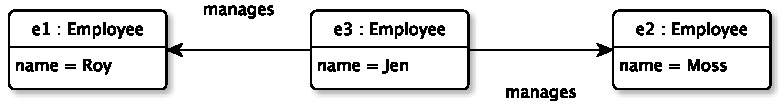
\includegraphics[width=\linewidth]{initial_chart_0}
	\caption{Initial version of the organisational chart model.}
	\label{fig:initial_chart_0}
\end{figure}

\begin{figure}[ht]
	\centering
	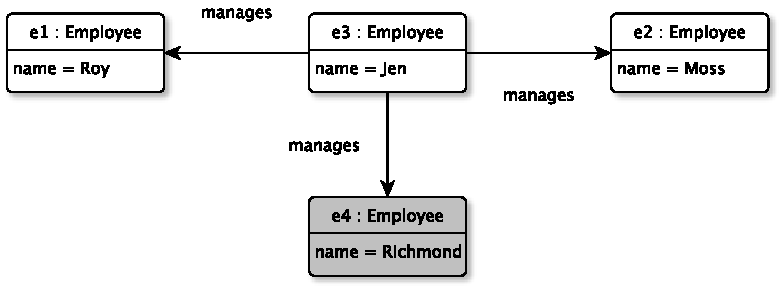
\includegraphics[width=\linewidth]{modified_chart}
	\caption{Modified version of the organisational chart model of Fig. \ref{fig:initial_chart}.}
	\label{fig:modified_chart}
\end{figure}

To illustrate the proposed approach, List. \ref{lst:xmimodel_0} shows a state-based representation of the model of Fig. \ref{fig:modified_chart} in (simplified) XMI, and List. \ref{lst:cbpmodel_0} shows the proposed equivalent change-based representation of the same model. Instead of a snapshot of the state of the model, the representation of List. \ref{lst:cbpmodel_0} captures the complete sequence of change events (create/set/add/remove/delete) that were performed on the model since its creation, organised in editing sessions (2 editing sessions in the case of this model). Replaying these changes produces the same state as the one captured in List. \ref{lst:xmimodel}, so the proposed representation carries at least as much information as the state-based representation.

\begin{lstlisting}[style=xmi,caption={State-based representation of the model of Figure \ref{fig:modified_chart} in (simplified) XMI.},label=lst:xmimodel_0]
<Employee xmi:id="e2" name="Jen">
<manages xmi:id="e1" name="Roy"/>
<manages xmi:id="e3" name="Moss"/>
<manages xmi:id="e4" name="Richmond"/>
</Employee>
\end{lstlisting}

\begin{figure}[h]
	\begin{lstlisting}[style=xml,caption={Change-based representation of the model of Figure \ref{fig:modified_chart}.},label=lst:cbpmodel_0]
	<session id="s1"/>
	<create eclass="Employee" epackage="employee" id="0"/>
	<add-to-resource position="0"><value eobject="0"/></add-to-resource>
	<set-eattribute name="name" target="0"><value literal="Roy"/></set-eattribute>
	<create eclass="Employee" epackage="employee" id="1"/>
	<add-to-resource position="1"><value eobject="1"/></add-to-resource>
	<set-eattribute name="name" target="1"><value literal="Jen"/></set-eattribute>
	<create eclass="Employee" epackage="employee" id="2"/>
	<add-to-resource position="2"><value eobject="2"/></add-to-resource>
	<set-eattribute name="name" target="1"><value literal="Moss"/></set-eattribute>
	<remove-from-resource><value eobject="0"/></remove-from-resource>
	<add-to-ereference name="manages" position="0" target="1"><value eobject="0"/></add-to-ereference>
	<remove-from-resource><value eobject="2"/></remove-from-resource>
	<add-to-ereference name="manages" position="1" target="1"><value eobject="2"/></add-to-ereference>
	<session id="s2"/>
	<create eclass="Employee" epackage="employee" id="3"/>
	<add-to-resource position="1"><value eobject="3"/></add-to-resource>
	<set-eattribute name="name" target="3"><value literal="Richmond"/></set-eattribute>
	<remove-from-resource><value eobject="3"/></remove-from-resource>
	<add-to-ereference name="manages" position="2" target="2"><value eobject="3"/></add-to-ereference>
	\end{lstlisting}
\end{figure}

Such a representation is particularly suitable for change-detection. For example, if the model had been modified in the editing session \emph{s1}, further changes of the model can be readily identified since then (i.e. in session \emph{s2} –- lines 15-20) instead of having to rediscover them through (expensive) state-based model differencing.

\section{Prototype Implementation of Change-Based Persistence}
\label{sec:prototype_implementation_of_change-based_persistence}
This work has implemented a prototype\footnote{The prototype is available under \url{https://github.com/epsilonlabs/emf-cbp}.} of the change-based model persistence format using the notification facilities provided by the Eclipse Modelling Framework. The implementation uses \emph{ChangeEventAdapter}, a subclass of EMF's \emph{EContentAdapter}, to receive and record \emph{Notification} events produced by the framework for every model-element level change.

\begin{figure}[th]
	\centering
	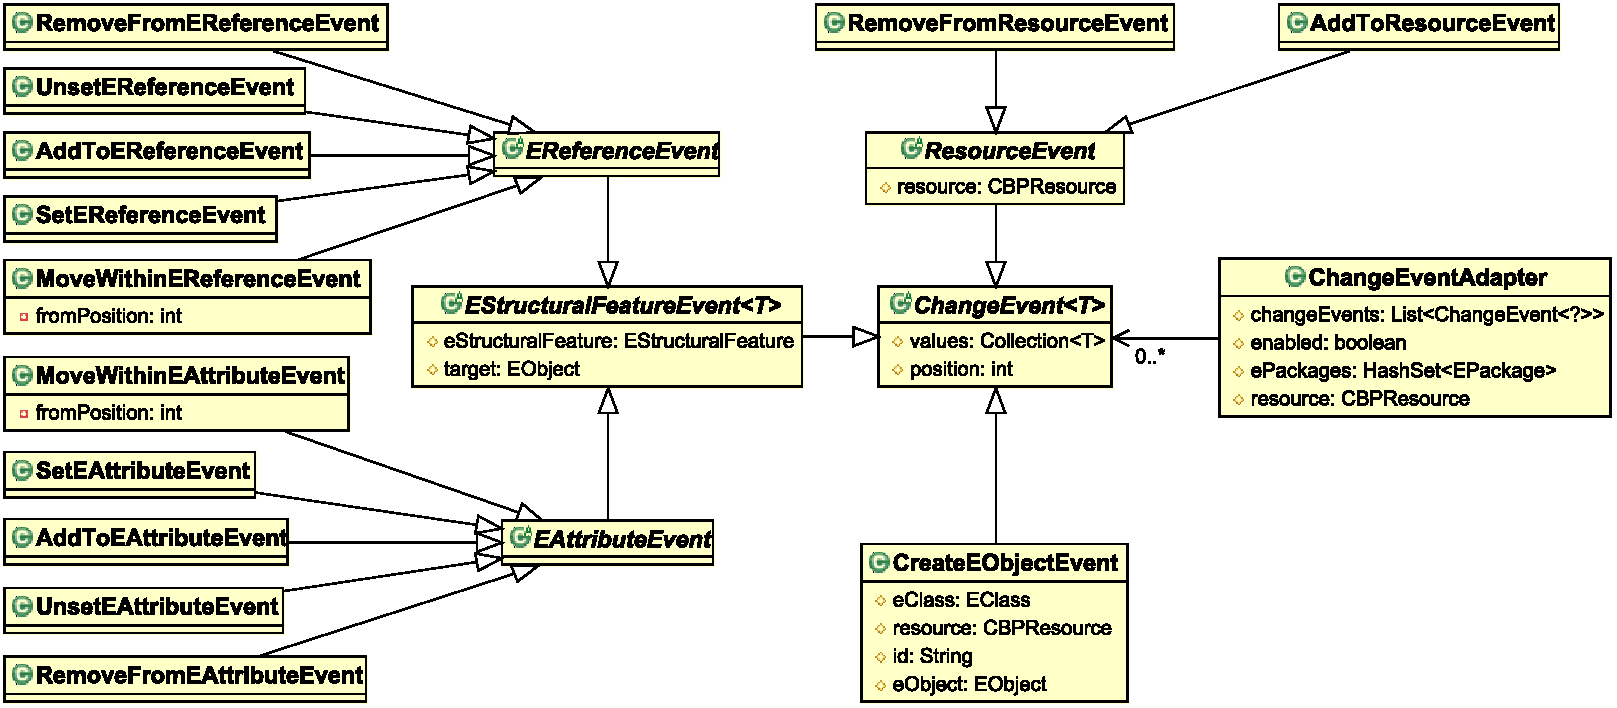
\includegraphics[width=\linewidth]{events}
	\caption{Event classes to represent changes of models.}
	\label{fig:events}
\end{figure}

Since not all change events are relevant to change-based persistence (e.g. EMF also produces change notifications when listeners/adapted are added/removed from the model), this work has defined a set of event classes to represent events of interest. The event classes are depicted in Fig. \ref{fig:events} as subclasses of the \emph{ChangeEvent} abstract class. 

The \emph{ChangeEvent} class has a multi-valued \emph{values} attribute which can accommodate both single-valued (e.g. set/add) or mutli-valued events (e.g. addAll/removeAll). \emph{ChangeEvent} can also accommodate different types of values, such as \emph{EObject}s for \emph{EReferenceEvents}, and primitive values (e.g. Integer, String) for \emph{EAttributeEvents}. The \emph{ChangeEvent} class also has a position attribute to hold the index of an \emph{EObject} or a literal when they are added to a \emph{Resource}, \emph{EReference}, or \emph{EAttribute} with multiple values (Lst. \ref{lst:cbpmodel}, line 3, 6, 9, 12, 14, 17, 20). 

Every time an \emph{EObject} is added to the model, a \emph{CreateEObjectEvent} and an \emph{AddToResourceEvent} are recorded (lines 2-3, 5-6, 8-9, and 16-17 in Lst. \ref{lst:cbpmodel}). When an EObject is deleted, or moved to a containment \emph{EReference} deeper in the model (Lst. \ref{lst:cbpmodel}, line 12, 14, 20), a \emph{RemoveFromResourceEvent} (Lst. \ref{lst:cbpmodel}, line 11, 13, 19) is recorded.

The \emph{ChangeEventAdapter} receives EMF change notifications in its \emph{notifyChanged()} method and filters and transforms them into appropriate change events. As an example of how notifications are filtered and transformed, Listing \ref{lst:javacode} shows how the implementation handles \emph{Notification.UNSET} events based on the type of the changed feature i.e. an \emph{UnsetEAttributeEvent} is instantiated if the feature of the notifier is an \emph{EAttribute}, or an \emph{UnsetEReferenceEvent} is created if the notifier is an \emph{EReference}. The transformed instances are then stored into a list of events in \emph{ChangeEventAdapter} (\emph{changeEvents}) for persistence. 

\begin{lstlisting}[style=java,caption={Simplified Java code to handle notification events.},label=lst:javacode]
public class ChangeEventAdapter extends EContentAdapter {
    ...
    @override
    public void notifyChanged(Notification n) {
        ...
        switch (n.getEventType()) {
        ... // other events
        case Notification.UNSET: {
            if (n.getNotifier() instanceof EObject) {
                EStructuralFeature feature = (EStructuralFeature) n.getFeature();
                if (feature instanceof EAttribute) {
                    event = new UnsetEAttributeEvent();
                } else if (feature instanceof EReference) {
                    event = new UnsetEReferenceEvent();
                }
            } break;
        } 
        ... // other events
\end{lstlisting}

\begin{figure}[th]
	\centering
	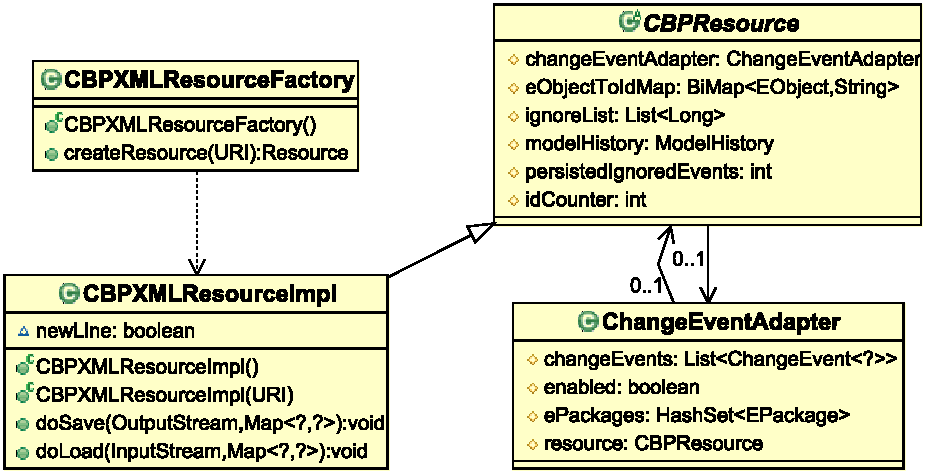
\includegraphics[width=0.6\linewidth]{resources}
	\caption{Factory, resources, and ChangeEventAdapter classes.}
	\label{fig:resources}
\end{figure}

To integrate seamlessly with the EMF framework and to eventually support multiple concrete change-based serialisation formats (e.g. XML-formatted representation for readability and binary for performance/size), the implementation has created the \emph{CBPResource} abstract class, that extends EMF's built-in \emph{ResourceImpl} class. The role of the abstract class is to encapsulate all change recording functionality while the role of its concrete subclasses is to implement serialisation and de-serialisation. For example, \emph{CBPXMLResourceImpl} persists changes in a line-based format where every change is serialised as a single-line XML document. In this way, when a model changes, The implementation can append the new changes to the end of the model file without needing to serialise the entire model again. The implementation has also implemented a \emph{CBPXMLResourceFactory} class that extends EMF's \emph{ResourceFactoryImpl}, as the factory class for change-based models. Figure \ref{fig:resources} shows the relationships between these classes.

\section{Load Time Reduction of Change-Based Models}
\label{sec:load_time_reduction_of_change-based_models}

\subsection{Running Example}
\label{subsec:case_study}
To explain change-based model persistence and the contribution of this work, the minimal tree metamodel is used (expressed in the Eclipse Modelling Framework's Ecore metamodelling language) and model illustrated in Figures \ref{fig:tree_metamodel} and \ref{fig:initial_model}.
EMF/Ecore was selected as the de-facto standard for object-oriented metamodelling, and this contrived example to avoid unnecessary repetition in the discussion, while providing a reasonable coverage of the core features of Ecore (classes, single/multi-valued features, references and attributes).
In this example, tree models consist of named nodes which can -- optionally -- contain other nodes (\emph{children} reference).

\begin{figure}[ht]
	\begin{subfigure}[t]{0.4\linewidth}
		\centering
		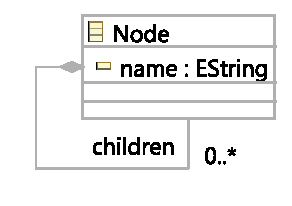
\includegraphics[width=0.8\linewidth]{node_metamodel}
		\caption{The tree metamodel.}
		\label{fig:tree_metamodel}
	\end{subfigure}
	\hfill
	\begin{subfigure}[t]{0.6\linewidth}
		\centering
		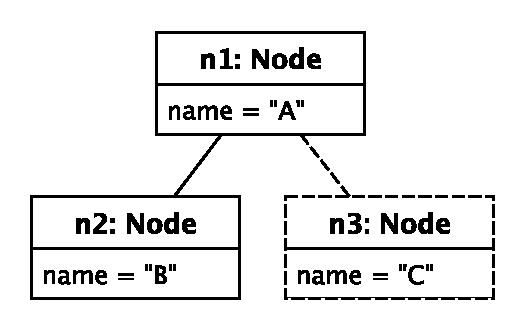
\includegraphics[width=0.6\linewidth]{initial_chart}
		\caption{A model that conforms to the tree metamodel (n3 was created and then deleted)}
		\label{fig:initial_model}
	\end{subfigure}
	\caption{A tree metamodel and its model as the running example.}
	\label{fig:append_speed}
\end{figure}

\noindent
\begin{minipage}[t]{0.5\linewidth}
	\begin{lstlisting}[style=xmi,caption={State-based representation of the tree model in (simplified) XMI.},label=lst:xmimodel]
	<Node id="n1" name="A">
	<children id="n2" name="B"/>
	</Node>
	\end{lstlisting}
\end{minipage}
\hfill
\begin{minipage}[t]{0.5\linewidth}
	\begin{lstlisting}[style=eol,caption={Change-based representation of the tree model.},label=lst:cbpmodel]
	create n1 of Node
	set n1.name to "A"      
	create n2 of Node
	set n2.name to "B"      
	create n3 of Node
	set n3.name to "C"      
	add n2 to n1.children   
	add n3 to n1.children
	remove n3 from n1.children   
	delete n3
	\end{lstlisting}
\end{minipage}

The model in Fig. \ref{fig:initial_model} consists of two nodes \emph{n1}, \emph{n2}.
The construction of the model starts with creating and naming three nodes (\emph{n1}, \emph{n2} and \emph{n3}).
Nodes \emph{n2} and \emph{n3} were then added as children of \emph{n1}.
Finally, node \emph{n3} was deleted from the model.
The final state of the model is presented in a simplified (state-based) XMI representation in Listing \ref{lst:xmimodel}.

In contrast to the state-based representation, a CBP representation of the model is illustrated in Listing \ref{lst:cbpmodel} (the syntax is a simplified version of the one introduced in\,\cite{yohannis2017turning}).
Lines 1-6 record the creation and naming of the three nodes, lines 7 and 8 record the addition of \emph{n2} and \emph{n3} as children of \emph{n1} and lines 9-10 capture the deletion of \emph{n3} (deletion effectively involves a removal and a deletion event).

For small changes made to large models, this approach can be beneficial since only the change events that need to be persisted every time -- as opposed to the entire model. However, loading the model by naively replaying all the events is not optimal particularly for models with long editing histories where prior events are often superseded by subsequent events. For example, creating \emph{n3} in line 5, naming it in line 6, and adding it to the children of \emph{n1} in line 8 are cancelled by the subsequent deletion of \emph{n3} in line 10. As such, the events in lines 5, 6, 8, 9 and 10 could be ignored during the loading process without affecting the eventual state of the model.

The flowchart in Fig. \ref{fig:flowchart} provides an overview of the editing lifecycle of a CBP model, and the artefacts and data structures involved in it. It also highlights (starred blocks) the extensions proposed compared to the original CBP approach in \cite{yohannis2017turning}.

In the original CBP approach, a model editing session involves three activities: loading a model, editing it, and saving new changes back to the model file\footnote{After saving a model, the user can make further changes and save it again.}. Loading is achieved by reading and replaying a sequence of change events stored in a CBP-formatted file. During the editing process, changes to the model are stored in a memory-based data structure (``Change events''), which are serialised and appended at the end of the CBP-formatted model file, and then flushed from memory, every time the model is saved.

\begin{figure}[ht]
	\centering
	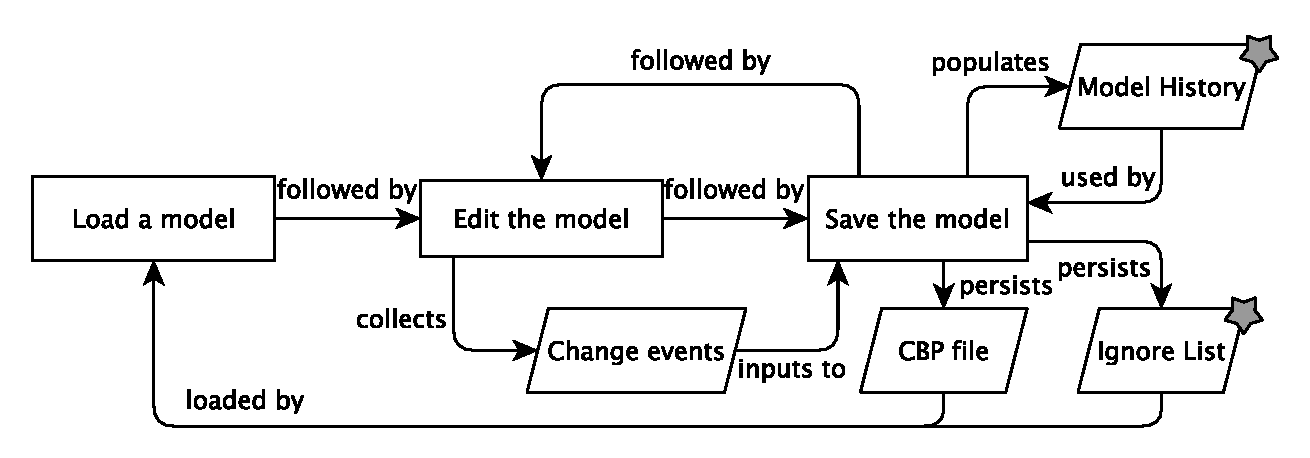
\includegraphics[width=\linewidth]{flowchart}
	\caption{The context flowchart of optimising loading performance of CBP.}
	\label{fig:flowchart}
\end{figure}

The proposed approach adds two new artefacts: a ``Model History'' data structure which is populated with change events and which is used to detect superseded events prior to saving, and an ``Ignore List'' file for each CBP model, which persists the position (i.e. line numbers) of superseded events so that they can be ignored the next time the model is loaded.

\subsection{Model History}
\label{subsec:model_history}
The proposed approach uses a data structure that memorises elements' events and their position (line number) in a CBP representation so it can reason about the events of a particular element and determine which of them are superseded. For the rest of the discussion the line number in the CBP representation is referred to as the \emph{event number}. The proposed data structure is presented in Fig. \ref{fig:object_history} as a class diagram.  

\begin{figure}[ht]
	\centering
	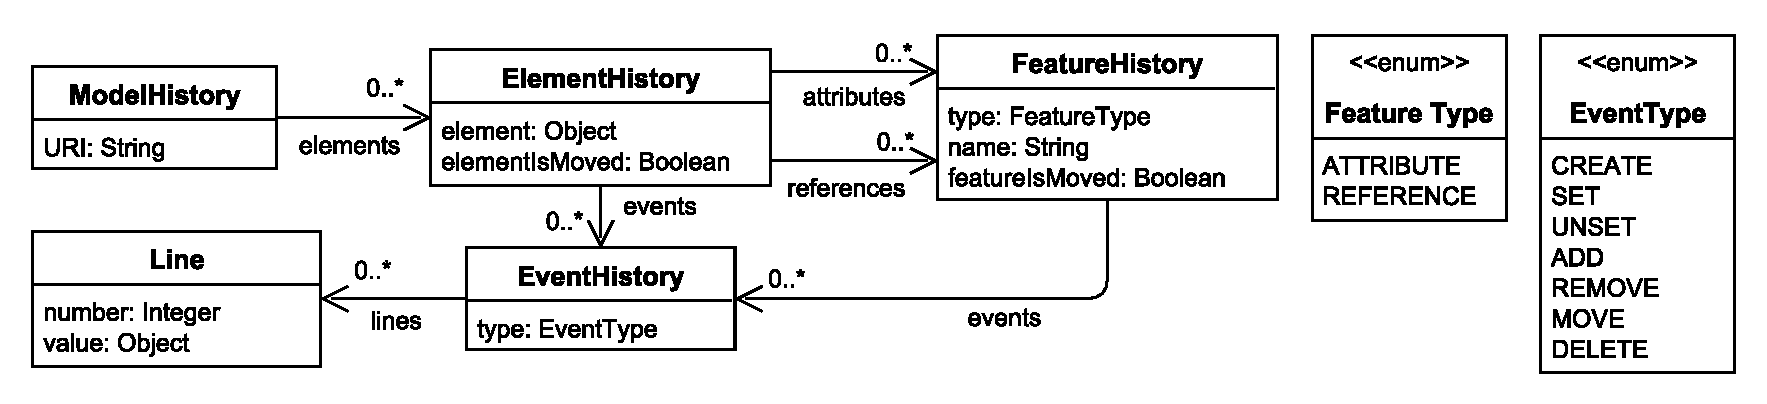
\includegraphics[width=\linewidth]{object_history}
	\caption{The class diagram of Model History.}
	\label{fig:object_history}
\end{figure}

\begin{figure}[ht]
	\centering
	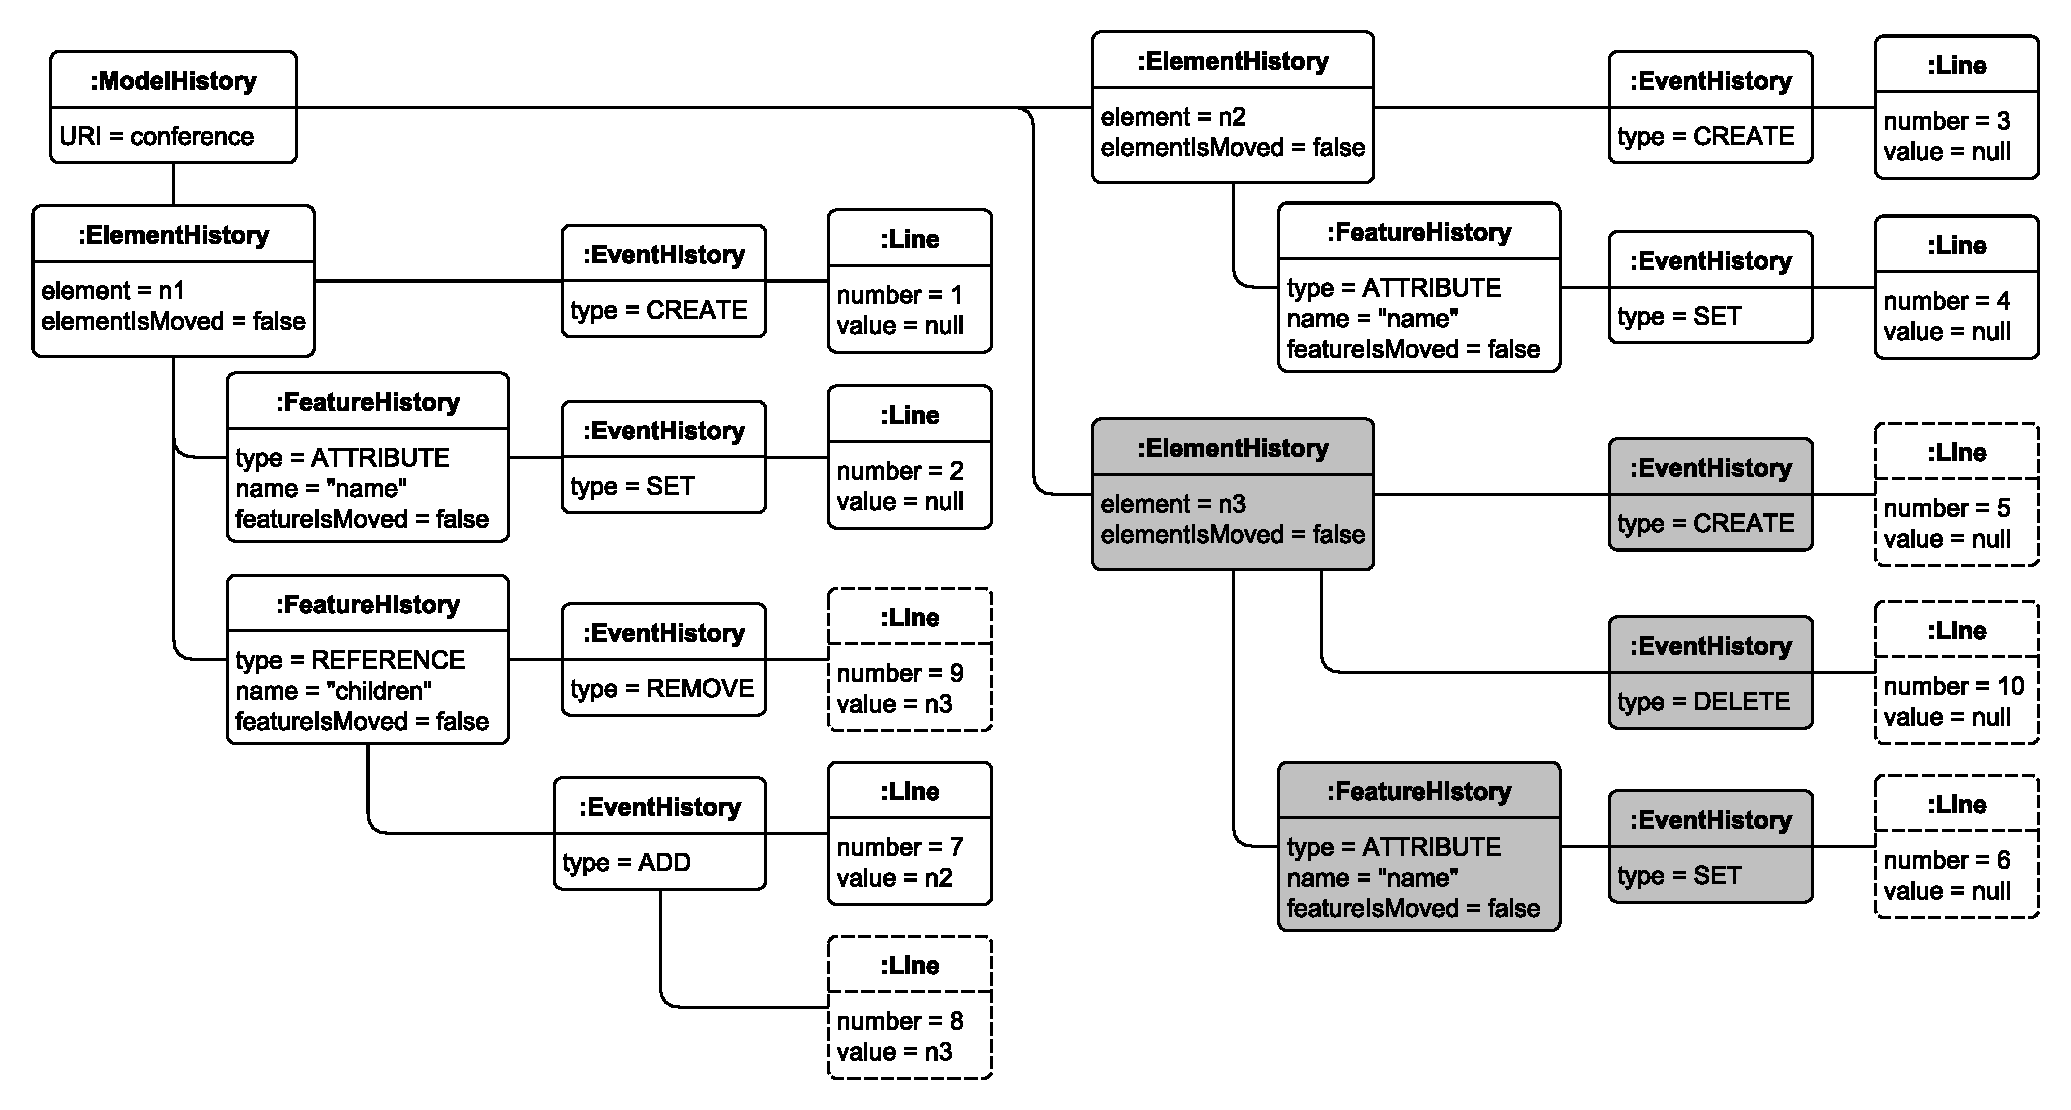
\includegraphics[width=\linewidth]{history_structure}
	\caption{The object diagram of the model history of the CBP model in Listing \ref{lst:cbpmodel}.}
	\label{fig:history_structure}
\end{figure}

A \emph{ModelHistory} has a \emph{URI} attribute to identify the model for which it records changes and can have many \emph{ElementHistory} elements. An \emph{ElementHistory} has an \emph{element} field that identifies the element that it refers to and an \emph{elementIsMoved} boolean flag. The  \emph{elementIsMoved} flag is used to indicate a \emph{move} event for the element (Sect. \ref{subsec:add_remove_and_move_operations} provides details of its use). Every \emph{ElementHistory} can have many \emph{FeatureHistories} to represent the editing histories of individual features (i.e. references/attributes) of the element.  A \emph{FeatureHistory} has three fields: \emph{type} to identify the feature's type (attribute or reference), \emph{name} to identify the feature's name, and \emph{featureIsMoved} that has the same role as attribute \emph{elementIsMoved} in \emph{ElementHistory}.

An \emph{EventHistory} represents series of events of the same type in the CBP model. An \emph{EventHistory} has an attribute \emph{type} to identify the events' type and can have many \emph{Line}s. A \emph{Line} has a \emph{number} attribute to store the event number in the CBP model and a \emph{value} that is used to store the element involved in the event (it is only used for \emph{ADD}, \emph{REMOVE} and \emph{MOVE} events).

Each \emph{FeatureHistory} can have many \emph{EventHistories} to represent the events that modify the value of the feature. Each \emph{ElementHistory} can have many \emph{EventHistories} to represent events that affect the state of the element (life-cycle and relations to multivalued features).

Fig. \ref{fig:history_structure} shows the object diagram of the model history of the CBP model in Listing \ref{lst:cbpmodel}. The grey rectangles are \emph{History} objects related to the deleted node \emph{n3}. The rectangles with the dashed outline are \emph{Line} objects that represent superseded changes. The next sections present the algorithms that use the information stored in the model history data structure to identify events that have no impact in the final state of the model, i.e. superseded events. The algorithms produce the ignore list that is used in the proposed CBP loading algorithm.

\subsection{Set and Unset Events}
\label{subsec:set_and_unset_events}
During the lifecycle of a model, a single-valued feature can be assigned many times. Each of the assignments is persisted as an event in the CBP model. However, only the last assigned value is necessary to obtain the current state of the feature.  That is, all events but the last can be ignored. For example, in Listing \ref{lst:set_unset_example}, the feature \emph{name} is assigned the ``A" value, nullified (unset), and finally assigned the ``B" value. That is, in the last state of the model: \emph{n1.name = ``B"}. As a result, the loading process could ignore all previous change events (lines 2 and 3) and only replay the last assignment event (line 4). 

\begin{lstlisting}[style=eol,caption={The CBP representation of attribute \emph{name} assignments.},label=lst:set_unset_example]
create n1 of Node
set n1.name to "A"
unset n1.name
set n1.name to "B"
\end{lstlisting}

The algorithm that identifies superseded \emph{SET} and \emph{UNSET} events for a feature is presented in Alg. \ref{alg:set_unset_optimisation}. The algorithm has two inputs: a list of event numbers of \emph{SET} events and a list of event numbers of \emph{UNSET} events. The output of the algorithm is an \emph{ignoreList} that includes the event numbers that are superseded. The inputs lists can be trivially constructed from the model history data structure. For the \emph{name} feature in Listing \ref{lst:set_unset_example} these are: $setEventNumbers = \{2,4\}$ and $unsetEventNumbers = \{3\}$.

\begin{algorithm}[H]
	\begin{small}
		\SetKwInOut{Input}{input}
		\SetKwInOut{Output}{output}
		\Input{two lists of Integer $setEventNumbers$}
		\Output{a list of Integer $ignoreList$}
		\SetKwBlock{Beginn}{beginn}{ende}
		\Begin{
			$setLastLine$ $\leftarrow$ getLastLine($setEventNumbers$)\;
			$unsetLastLine$ $\leftarrow$ getLastLine($unsetEventNumbers$)\;
			\uIf{$setLastLine > unsetLastLine$}{
				$ignoreList \leftarrow (setEventNumbers \cup unsetEventNumbers) \setminus \{setLastLine\} $\;
			}
			\ElseIf{$setLastLine < unsetLastLine$}{
				$ignoreList \leftarrow (setEventNumbers \cup unsetEventNumbers)$\;
			}
			\Return{$ignoreList$}\;
		}
	\end{small}
	\caption{Algorithm to identify event numbers of superseded \emph{set} and \emph{unset} events}
	\label{alg:set_unset_optimisation}
\end{algorithm}

The \emph{ignoreList} is populated as follows.
In lines 2 and 3, the last event number of each input list is stored in \emph{setLastLine} and \emph{unsetLastLine} respectively. If $setLastLine > unsetLastLine$ (line 4) then $ignoreList = (setEventNumbers \cup unsetEventNumbers) \setminus  \{setLastLine\} $, i.e. all events except the last \emph{SET} event can be ignored. If $setLastLine < unsetLastLine$ (line 6) then $ignoreList = (setEventNumbers \cup unsetEventNumbers)$, i.e. all events can be ignored. For the \emph{name} feature in Listing \ref{lst:set_unset_example}, $ignoreList = \{2, 3\}$.

\subsection{Add, Remove, and Move Events}\label{subsec:add_remove_and_move_operations}
Similarly, the contents of a multi-valued feature can be modified many times. If the same element is added and removed multiple times,  only that last event is necessary to determine if the element should appear in the values of the feature. For example, in Listing \ref{lst:add_remove_move_reference},  nodes \emph{n2} and \emph{n3} are added to the \emph{children} feature of \emph{n1} (lines 4-5), and then \emph{n3} is removed (line 6). That is, in the last state of the model: \emph{n1.children = [n2]}. As a result, the loading process could ignore the events that represent the \emph{ADD} and \emph{REMOVE} events of \emph{n3}. So far, the algorithm only supports unique features (i.e. features that do not allow duplicate values). An extension to support duplicate values is part of this research's future work. 

\begin{lstlisting}[style=eol,caption={Example of CBP representation of attribute \emph{values}'s add and remove operations.},label=lst:add_remove_move_reference]
create n1 of Node
create n2 of Node
create n3 of Node
add n2 to n1.children
add n3 to n1.children
remove n3 from n1.children
\end{lstlisting}

The algorithm that identifies superseded \emph{ADD} and \emph{REMOVE} events for a feature is presented in Alg. \ref{alg:add_remove_move_optimisation}. The algorithm has four inputs: a list of Line objects of \emph{ADD} events, a list of Line objects of \emph{REMOVE} events, the element of interest and a flag that indicates a \emph{MOVE} event on the analysed feature.  The output of the algorithm is an \emph{ignoreList} that includes the event numbers that are superseded. The inputs lists can be easily constructed from the Model History data structure. For the \emph{children} feature in Listing \ref{lst:add_remove_move_reference} these are: $addEventLines=\{\{4,n2\},\{5,n3\}\}$, $removeEventLines=\{\{6,n3\}\}$, $moveEventLines=\emptyset$, $operandValue=n3$, and $featureIsMoved=\mathrm{False}$.

\begin{algorithm}[H]
	\begin{small}
		\SetKwInOut{Input}{input}
		\SetKwInOut{Output}{output}
		\SetKwProg{Struct}{struct}{}{end}
		\Struct{Line}{
			Integer $eventNumber$;
			Anytype $value$;
		}
		\Input{two lists of Line $addEventLines$, $removeEventLines$, a variable of Anytype $operandValue$, a variable of Boolean $featureIsMoved$} % and $moveEventLines$, , an variable of Feature $feature$}
		\Output{a list of Integer $ignoreList$}
		\SetKwBlock{Beginn}{beginn}{ende}
		\Begin{
			\If{$featureIsMoved$ = false}{
				$filteredAddLines$ $\leftarrow$ filterByValue($addEventLines$, $operandValue$)\;
				$filteredRemoveLines$ $\leftarrow$ filterByValue($removeEventLines$, $operandValue$)\;
				$addLastLine$ $\leftarrow$ getLastLine($filteredAddLines$)\;
				$removeLastLine$ $\leftarrow$ getLastLine($filteredRemoveLines$)\;
				\uIf{$addLastLine > removeLastLine$}{
					$ignoreList \leftarrow (filteredAddLines.eventNumber \cup filteredRemoveLines.eventNumber \setminus \{addLastLine\} $\;
				}
				\ElseIf{$addLastLine < removeLastLine$}{
					$ignoreList \leftarrow (filteredAddLines.eventNumber \cup filteredRemoveLines.eventNumber$\;
				}
			}
			\Return{$ignoreList$}\;
		}
	\end{small}
	\caption{Algorithm to identify event numbers of superseded \emph{add}, \emph{remove}, and \emph{move} events.}
	\label{alg:add_remove_move_optimisation}
\end{algorithm}

\noindent
\begin{minipage}[t]{0.48\linewidth}
	\begin{lstlisting}[style=eol,caption={The CBP representation of reference \emph{children}'s move event.},label=lst:move_attribute_example]
	create p of Node
	create n1
	create n2
	create n3
	add n1 to p.children
	add n2 to p.children
	add n3 to p.children
	move from 0 to 1 in p.children
	remove n2 from p.children
	\end{lstlisting}
\end{minipage}
\hfill
\begin{minipage}[t]{0.48\linewidth}
	\begin{lstlisting}[style=eol,caption={The effective CBP representation of reference \emph{children}'s move event.},label=lst:move_attribute_example_error]
	create p of Node
	create n1
	create n2
	create n3
	add n1 to p.children
	add n3 to p.children
	move from 0 to 1 in p.children
	\end{lstlisting}
\end{minipage}

The \emph{ignoreList} is populated as follows. If the flag \emph{featureIsMoved} is true then nothing is added to the list (the need for this flag is explained later in this section). If the flag \emph{featureIsMoved} is false, then lines 6 and 7 filter the $addEventLines$ and $removeEventLines$ to only keep Lines for which the \emph{value} is equal to \emph{operandValue}. The filtered lists are stored in $filteredAddLines$ and $filteredRemoveLines$ respectively. The rest of the algorithm works similar to Alg. \ref{alg:set_unset_optimisation}, ignoring all events but the last if it was an \emph{ADD}, else ignoring all events. 

The flag \emph{featureIsMoved} in line 5 in Alg. \ref{alg:add_remove_move_optimisation} is required to prevent ordering errors in the final state. As an illustration, the final states of the original CBP model presented in Listing  \ref{lst:move_attribute_example} and the effective CBP model of Listing \ref{lst:move_attribute_example_error} which \emph{does not} consider the \emph{featureIsMoved} flag are compared. In the effective CBP model, the events related to \emph{n2} have been ignored. Notice that the final state of the effective version is $p.values = [n3, n1]$  which is different from the original version $p.values = [n1, n3]$. The reason is that the move event in line 8 in the original version works on a different value than the one in the effective version.

\subsection{Create and Delete Events}
\label{subsec:create_and_delete_operations}
When an element is deleted, it is completely removed from the model. Therefore, all events (create, set, unset, move, add, remove, delete) related to the element that happened before the event can be ignored, including all events related to its features, unless the element has been moved. For example, when node \emph{n3} in Listing \ref{lst:cbpmodel}  is deleted, the events in lines 5-6 and 8-10 are superseded. The effective CBP model of Listing \ref{lst:cbpmodel} is presented in Listing \ref{lst:cbpmodel_optimised}.

\begin{lstlisting}[style=eol,caption={Change-based representation of the model of Fig. \ref{fig:initial_model} after removal of node \emph{n5}.},label=lst:cbpmodel_optimised]
create n1 of Node
set n1.name to "A"
create n2 of Node
set n2.name to "B"
add n2 to n1.children
\end{lstlisting}

\begin{algorithm}[H]
	\begin{small}
		\SetKwInOut{Input}{input}
		\SetKwInOut{Output}{output}
		\Input{a variable of Object $deletedElement$, a list of Integer $ignoreList$}
		\Output{a list of Integer $ignoreList$}
		\Begin{
			$elementIsMoved$ $\leftarrow$ isElementMoved($deletedElement$)\;
			\If{$elementIsMoved$ = false}{
				$eventHistoryList$ $\leftarrow$ getAllEventHistories($deletedElement$)\; 
				\ForEach{$eventHistory$ in $EventHistoryList$}{
					$lineList$ $\leftarrow$ getLines($eventHistory$)\;
					Add all event numbers in $lineList$ into $ignoreList$\; 
				}
				$featureList$ $\leftarrow$ getAllAttributes($deletedElement$)\;
				\ForEach{$attribute$ in $featureList$}{
					$eventHistoryList$ $\leftarrow$ getAllEventHistories($feature$)\;
					\ForEach{$eventHistory$ in $EventHistoryList$}{
						$lineList$ $\leftarrow$ getLines($eventHistory$)\;
						Add all event numbers in $lineList$ into $ignoreList$\; 
					}       
				}   
			}
			\Return{$ignoreList$}\;
		}
	\end{small}
	\caption{Algorithm to identify lines that are ignored after \emph{delete} events}
	\label{alg:create_delete_optimisation}
\end{algorithm}

The algorithm that identifies superseded events for a deleted element is presented in Alg. \ref{alg:create_delete_optimisation}. The algorithm has one input: the deleted element. The output of the algorithm is an \emph{ignoreList} that includes the event numbers that are superseded. The inputs lists can be trivially constructed from the model history data structure.

The algorithm starts by computing flag \emph{elementIsMoved} to determine whether the \emph{deletedElement} is already moved or not (line 2).
If it is false then it is safe to remove all lines that refer to the element (line 3) (the reason for using this flag was explained in section \ref{subsec:add_remove_and_move_operations}), otherwise, no action is taken. The algorithm then retrieves all event histories (\emph{eventHistoryList}) that refer to the element (line 4) and iterates through each event history (lines 5-8). For every event history (\emph{eventHistory} -- line 5), the algorithm retrieves its lines \emph{lineList} (line 6) and puts all their event numbers into the \emph{ignoreList} (line 7). After that, the algorithm continues to iterate through all its features and puts all lines' event numbers into the \emph{ignoreList} (lines 12-15). Finally, the algorithm returns the \emph{ignoreList} as its output.

\subsection{Performance Evaluation}
\label{subsec:performance_evaluation}
This work has developed the proposed efficient loading algorithm on top of the original CBP implementation from \cite{yohannis2017turning} and evaluated the algorithm's model loading performance, as well as its memory footprint and its impact on the time required to save changes made to CBP models. The evaluation was performed on Windows Server 2008 R2 64-bit with an Intel Xeon E5530 @2.40 GHz (2 processors) processor, 36 GB of memory, and the Java SE Runtime Environment (build 1.8.0\_66-b18).

\begin{figure}[htbp]
	\centering
	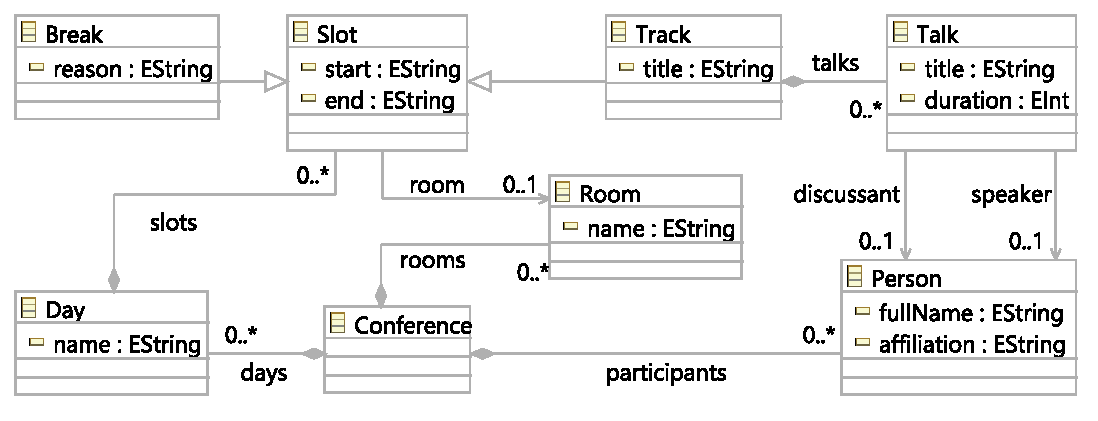
\includegraphics[width=0.9\linewidth]{conference_metamodel}
	\caption{The conference metamodel.}   
	\label{fig:node_metamodel}
\end{figure}

For the evaluation experiments, this work has used synthetic models of different sizes conforming to the \emph{conference} metamodel in Fig. \ref{fig:node_metamodel}. This work has selected this metamodel as it provides reasonable coverage of the features of the EMF modelling capabilities such as single- and multi-valued features, inheritance, and containment and non-containment references. This work had little option other than to use synthetic models for the experiments given that CBP is a very recent contribution and this work is not aware of any existing datasets containing real-world models expressed in a change-based format. Synthesising such models from existing state-based models (e.g. in XMI) was not an option either as state-based models do not capture editing-history-related information.    

\subsubsection{Loading Time}
\label{subsec:loading_time_test}

For this experiment, this work created and persisted change-based models of different sizes (from 500 up to 33,000 elements) conforming to the conference metamodel of Fig. \ref{fig:node_metamodel} through a random model generator that simulates the actions of a human modeller (i.e. creates/deletes elements, sets/unsets values of their features). This work then used the proposed and the baseline loading algorithms to reconstruct the state of these models and measured their execution time. The results are shown in Fig. \ref{fig:loading_speed_conf} and demonstrate the considerable time savings (up to 44\% faster compared to the original CPB implementation for the largest models) delivered by the proposed loading algorithm.

\begin{figure}[ht]	
	\begin{subfigure}[t]{0.5\linewidth}
		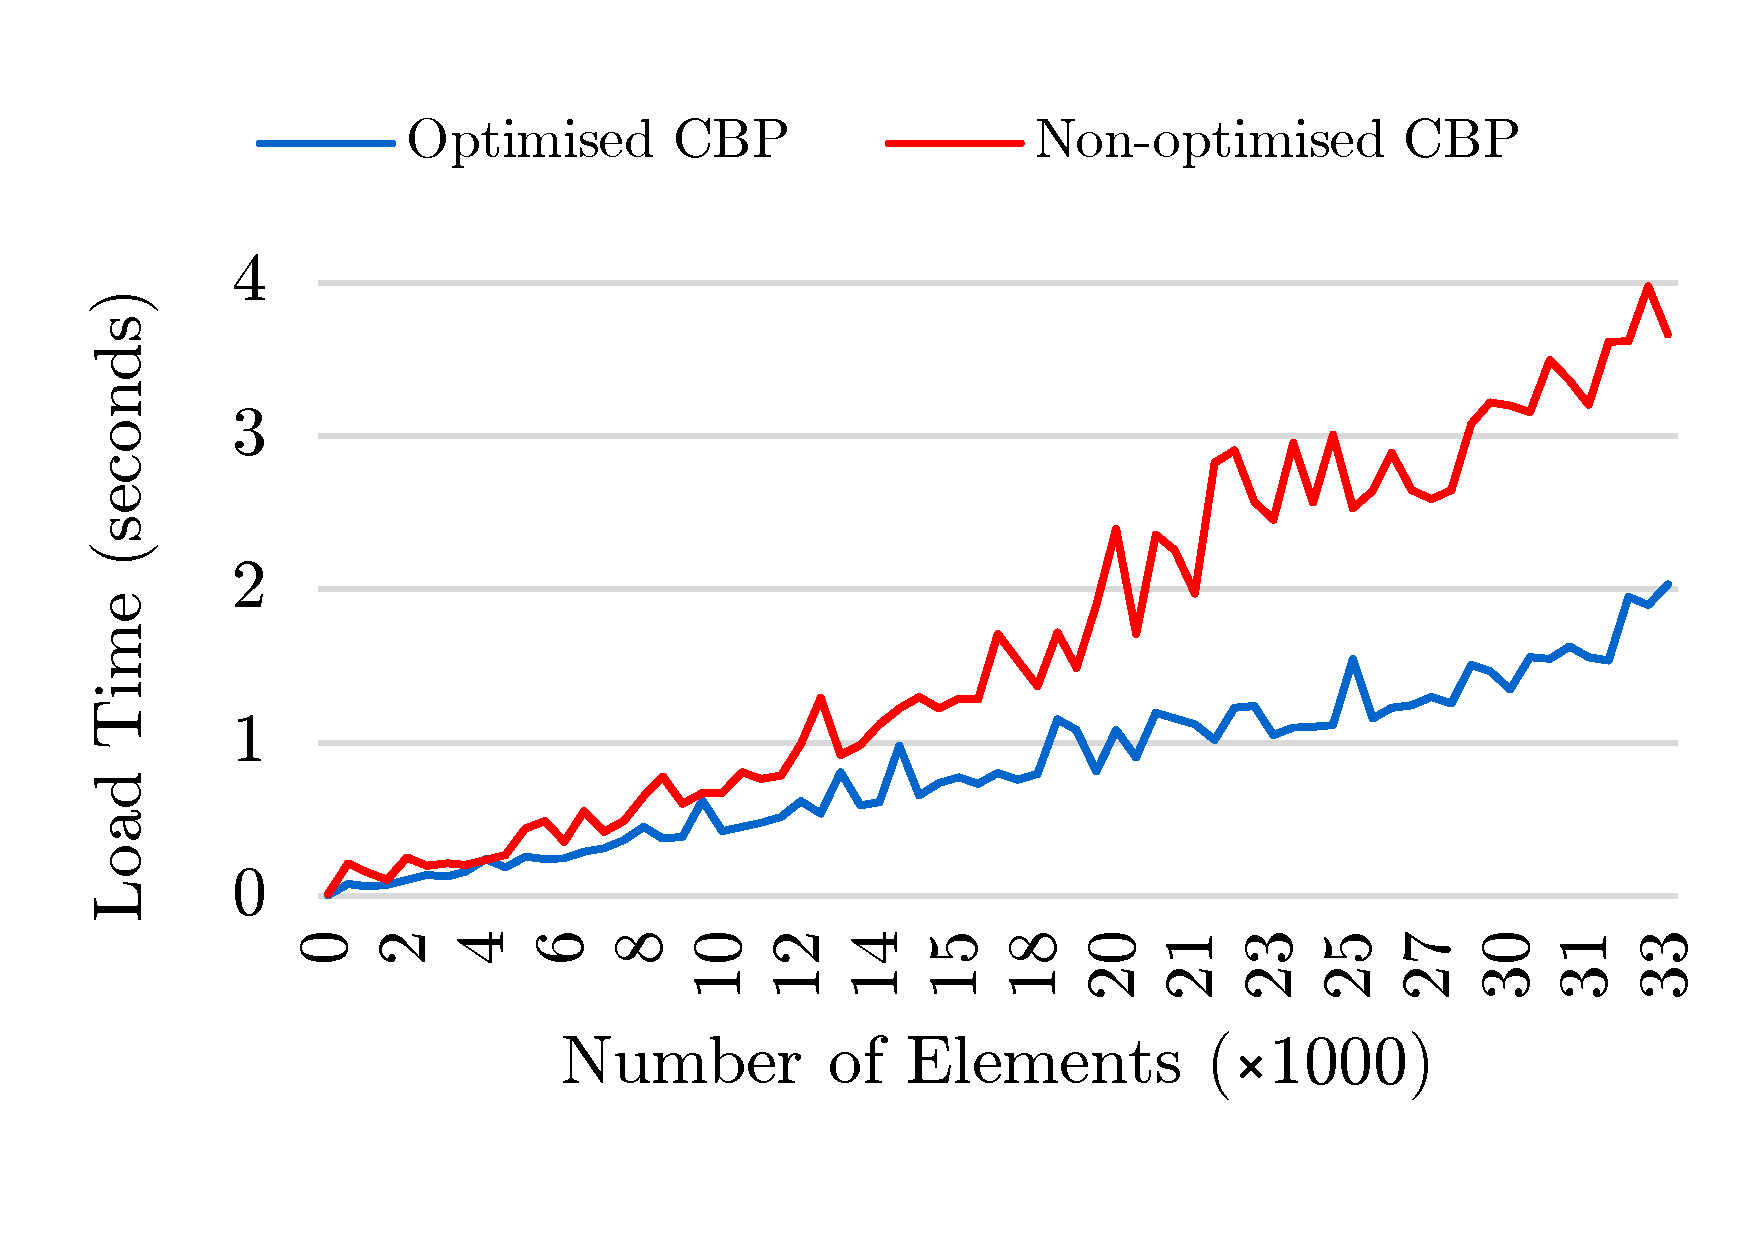
\includegraphics[width=\linewidth]{loading_speed_conf}
		\caption{Optimised CBP vs Non-optimised CBP}\label{fig:loading_speed_conf}
	\end{subfigure}
	\hfill
	\begin{subfigure}[t]{0.5\linewidth}
		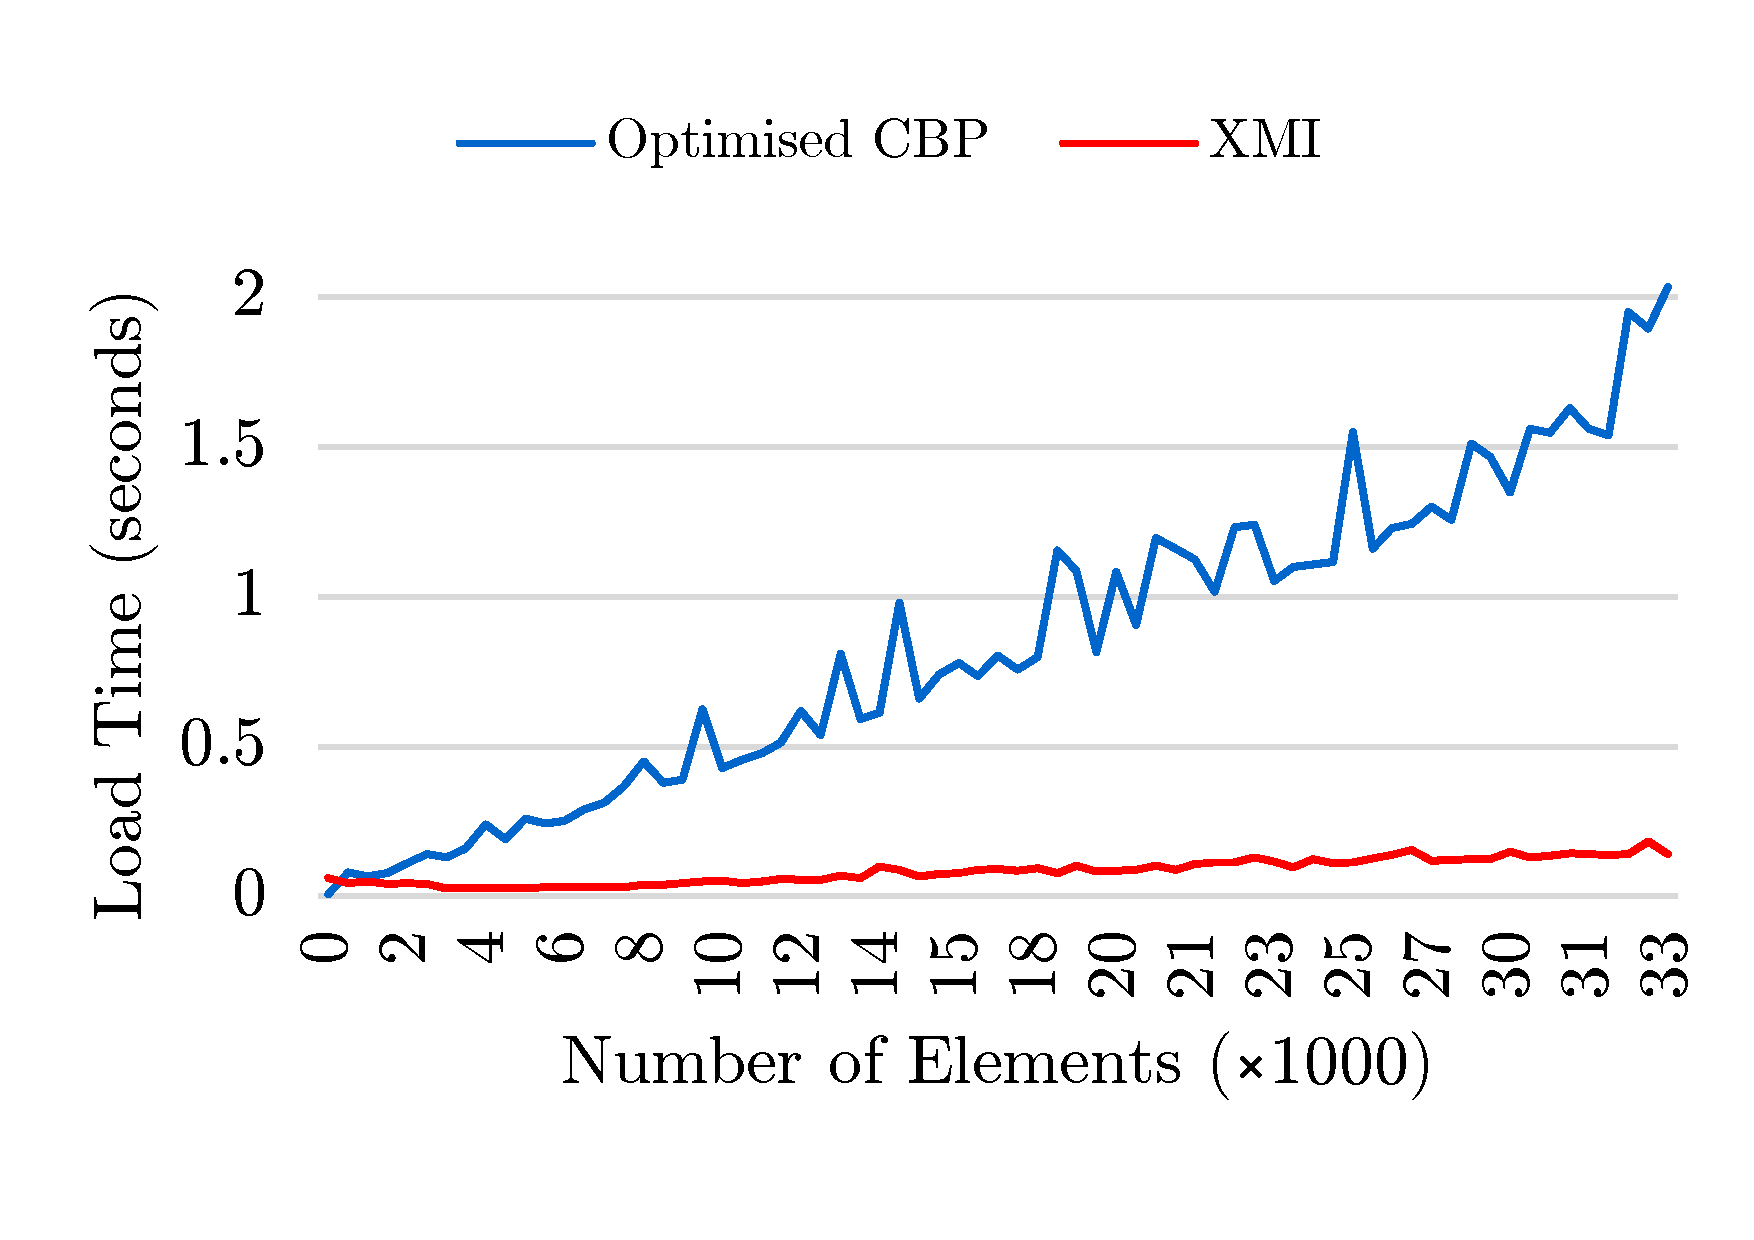
\includegraphics[width=\linewidth]{loading_speed_conf_ocbp_xmi}
		\caption{Optimised CBP vs XMI}\label{fig:loading_speed_conf_ocbp_xmi}		
	\end{subfigure}	
	\caption{A comparison on load time between optimised CBP, non-optimised CBP, and XMI.}
	\label{fig:loading_speed}
\end{figure}

For reference, this work also contrasts the execution time for the proposed algorithm against that of loading the equivalent state-based model in XMI. As can be observed in Fig. \ref{fig:loading_speed_conf_ocbp_xmi}, despite the improvements delivered by the new algorithm, loading change-based models is still roughly 10 times slower than their state-based counterparts. However, as discussed in\,\cite{yohannis2017turning}, this can be an acceptable trade-off considering the other benefits that change-based model persistence has the potential to offer (e.g. more precise differencing and hence more efficient incremental execution of model management programs and more effective model merging).

\subsubsection{Saving Time}
\label{subsec:saving_time_test}

To achieve the benefits in terms of loading time demonstrated in Section \ref{subsec:loading_time_test}, the algorithm requires additional work to be done (i.e. to assemble the model history data structure and compute the ignore list delta) during the model saving phase as discussed in Section \ref{subsec:case_study}. To assess the impact of this additional work on the overall time required to save changes in models, this work used a random model generator to build up multiple versions of a conference model through random sequences of creating, deleting and modifying model elements, starting with an empty model and growing it up to 21,000 elements. Every 100 new elements, the generator would save the changes and measure the time required for this activity to complete. This work repeated the experiment with the prototype, with the existing baseline CBP implementation and with state-based models stored in XMI.

\begin{figure}[ht]	
	\begin{subfigure}[t]{0.5\linewidth}
		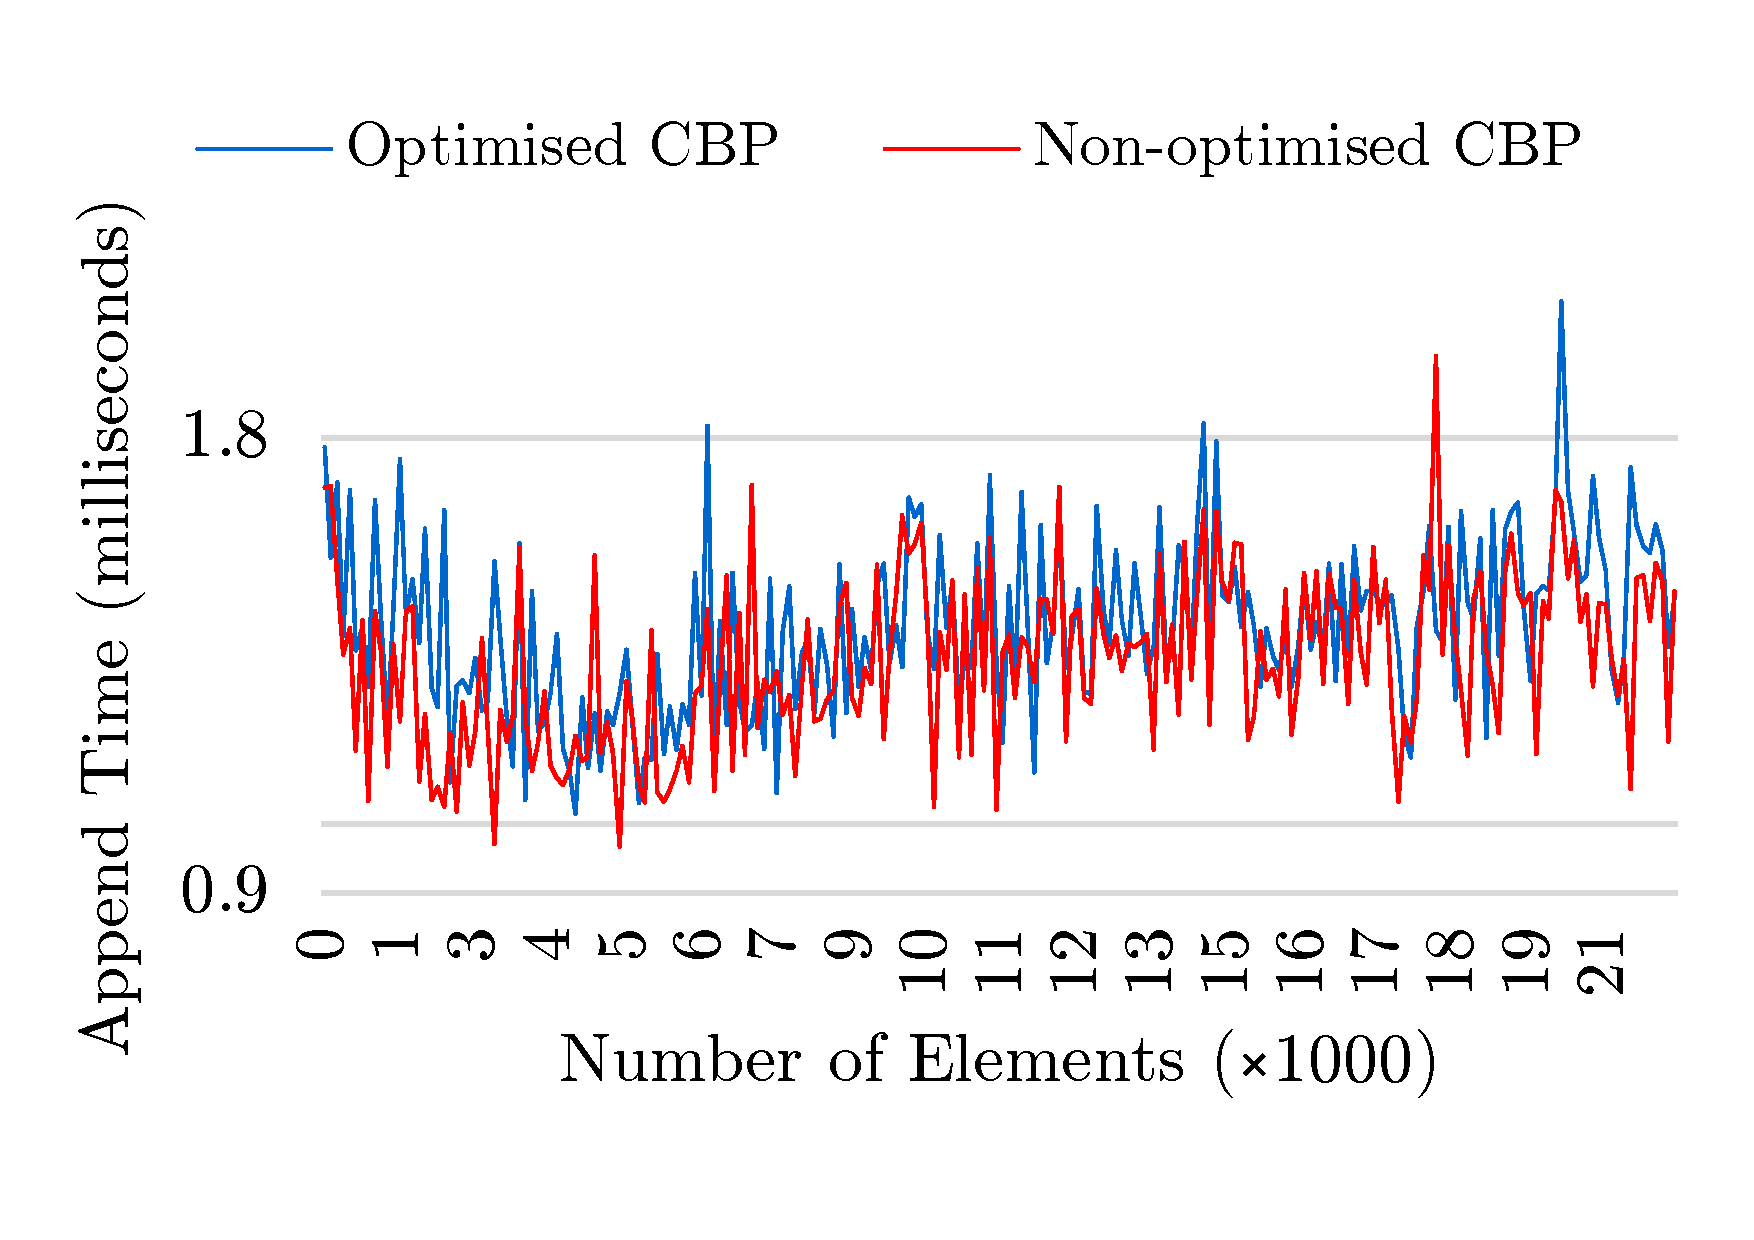
\includegraphics[width=\linewidth]{append_speed_conf}
		\caption{Optimised vs non-optimised CBPs}\label{fig:append_speed_conf}
	\end{subfigure}
	\hfill
	\begin{subfigure}[t]{0.5\linewidth}
		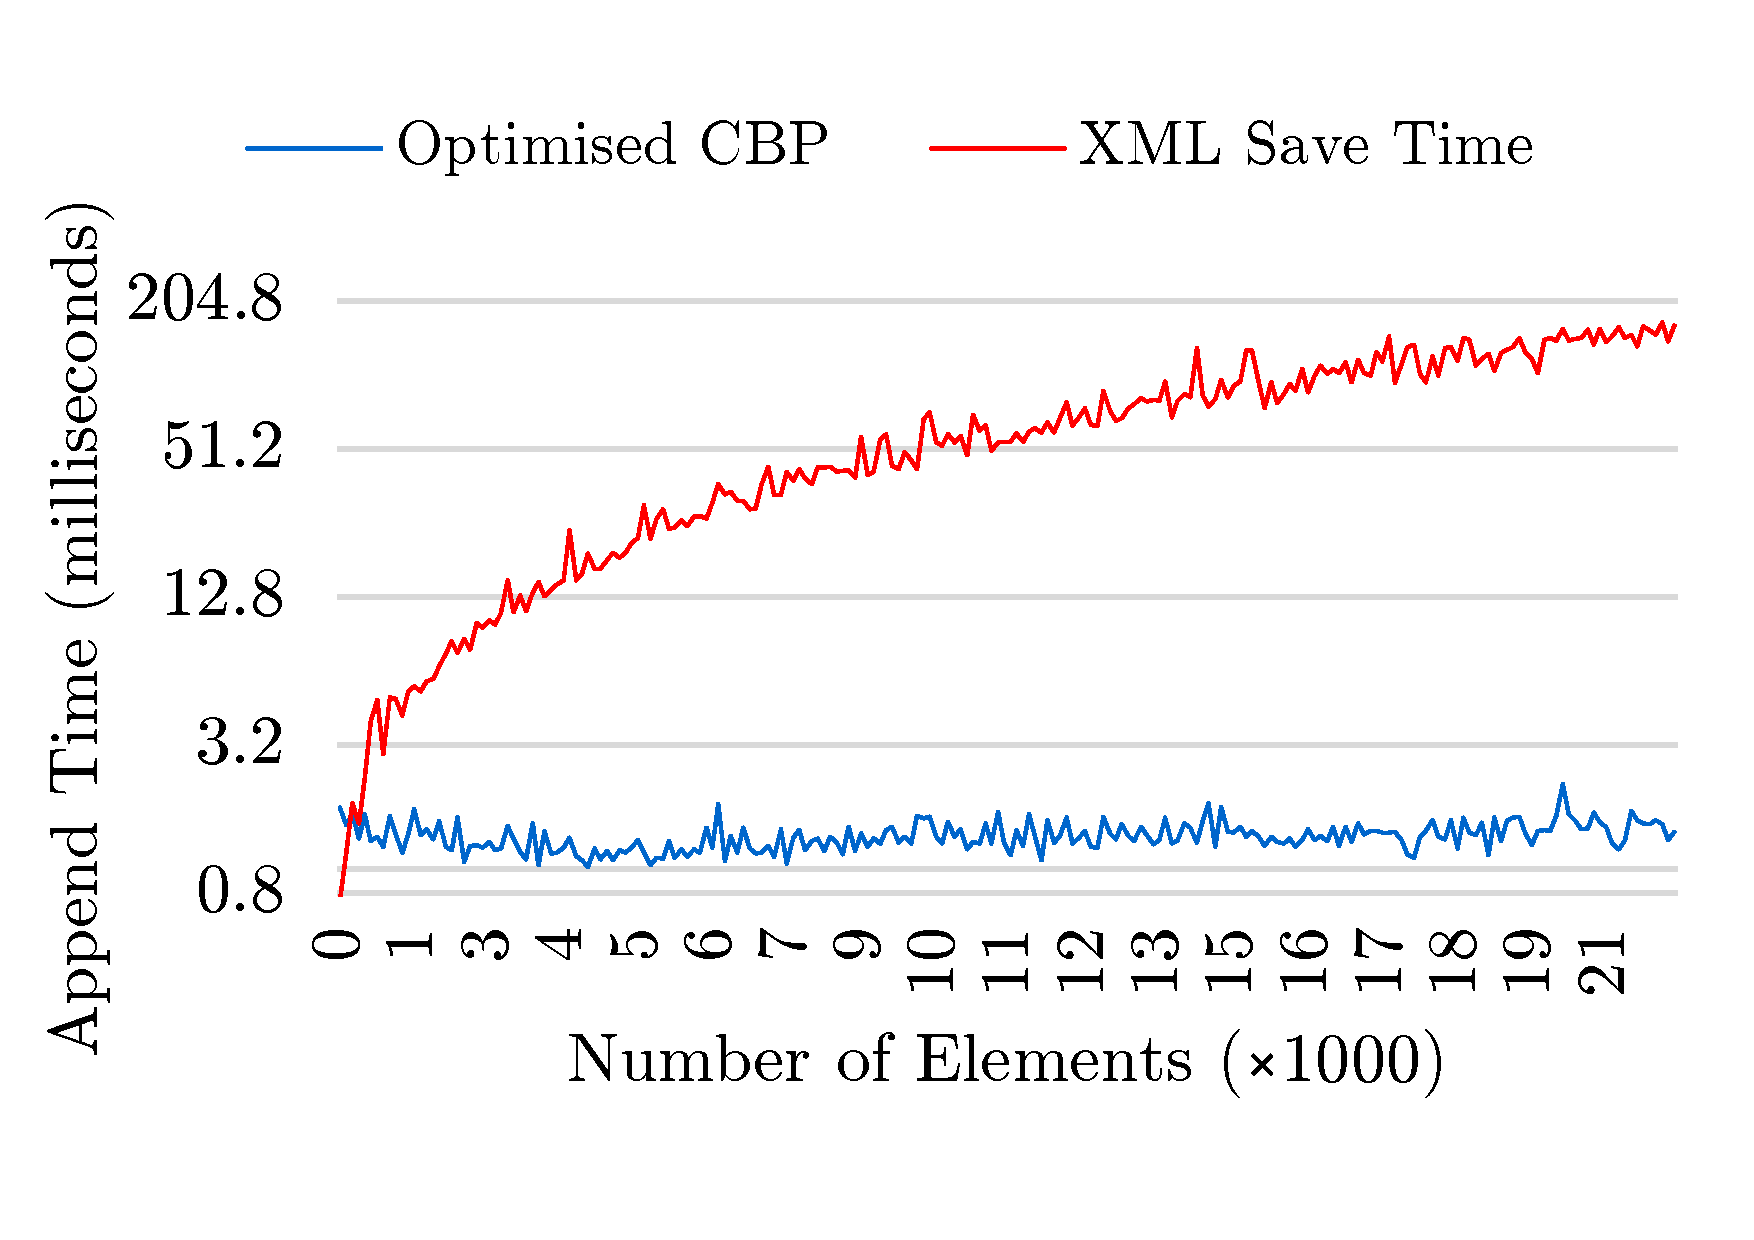
\includegraphics[width=\linewidth]{append_speed_conf_ocbp_xmi}
		\caption{Optimised CBP vs XMI}\label{fig:append_speed_conf_ocbp_xmi}		
	\end{subfigure}	
	\caption{A comparison on time used to persist models between optimised CBP, non-optimised CBP, and XMI. The y-axis is $log_2$ scaled.}
	\label{fig:append_speed}
\end{figure}

As shown in Fig. \ref{fig:append_speed_conf} the performance of the two CBP implementations is almost indistinguishable, which indicates that the cost of the extra work needed by the proposed algorithm at this stage is negligible. On the other hand, CBP implementations are significantly faster at saving changes than XMI. This is expected as the CBP implementations only need to save the last set of changes every time by appending them to the existing model file (and hence their performance is relative to the number of changes since last saved), while the XMI implementation needs to reconstruct an XML document for the entire state of the model and replace the contents of the model file every time (and hence its performance is relative to the size of the entire model). 

\subsubsection{Memory Footprint}
\label{subsec:memory_consumption}
As the proposed loading algorithm requires the maintenance of an additional in-memory data structure that keeps track of element and feature editing histories (see Fig. \ref{fig:history_structure}), This work conducted an additional experiment to measure its memory footprint. As with the experiment in Sect. \ref{subsec:saving_time_test}, this work used a random model generator to build up a conference model through random sequences of creating, deleting and modifying model elements, starting with an empty model and growing it up to 10,000 elements. Every 100 new elements, this work measured the memory consumed by the program. The results are plotted in Fig. \ref{fig:memory_ocbp_cbp_xmi} and demonstrate the significant overhead of the used data structure.

For reference, this work also includes the memory footprints of XMI in Fig. \ref{fig:memory_ocbp_cbp_xmi} to contrast it with both CBP implementations. As observed, XMI outperforms the optimised CBP representation and performs slightly better than the original CBP representation in terms of its memory footprint. 

\begin{figure}[H]	
	\centering
	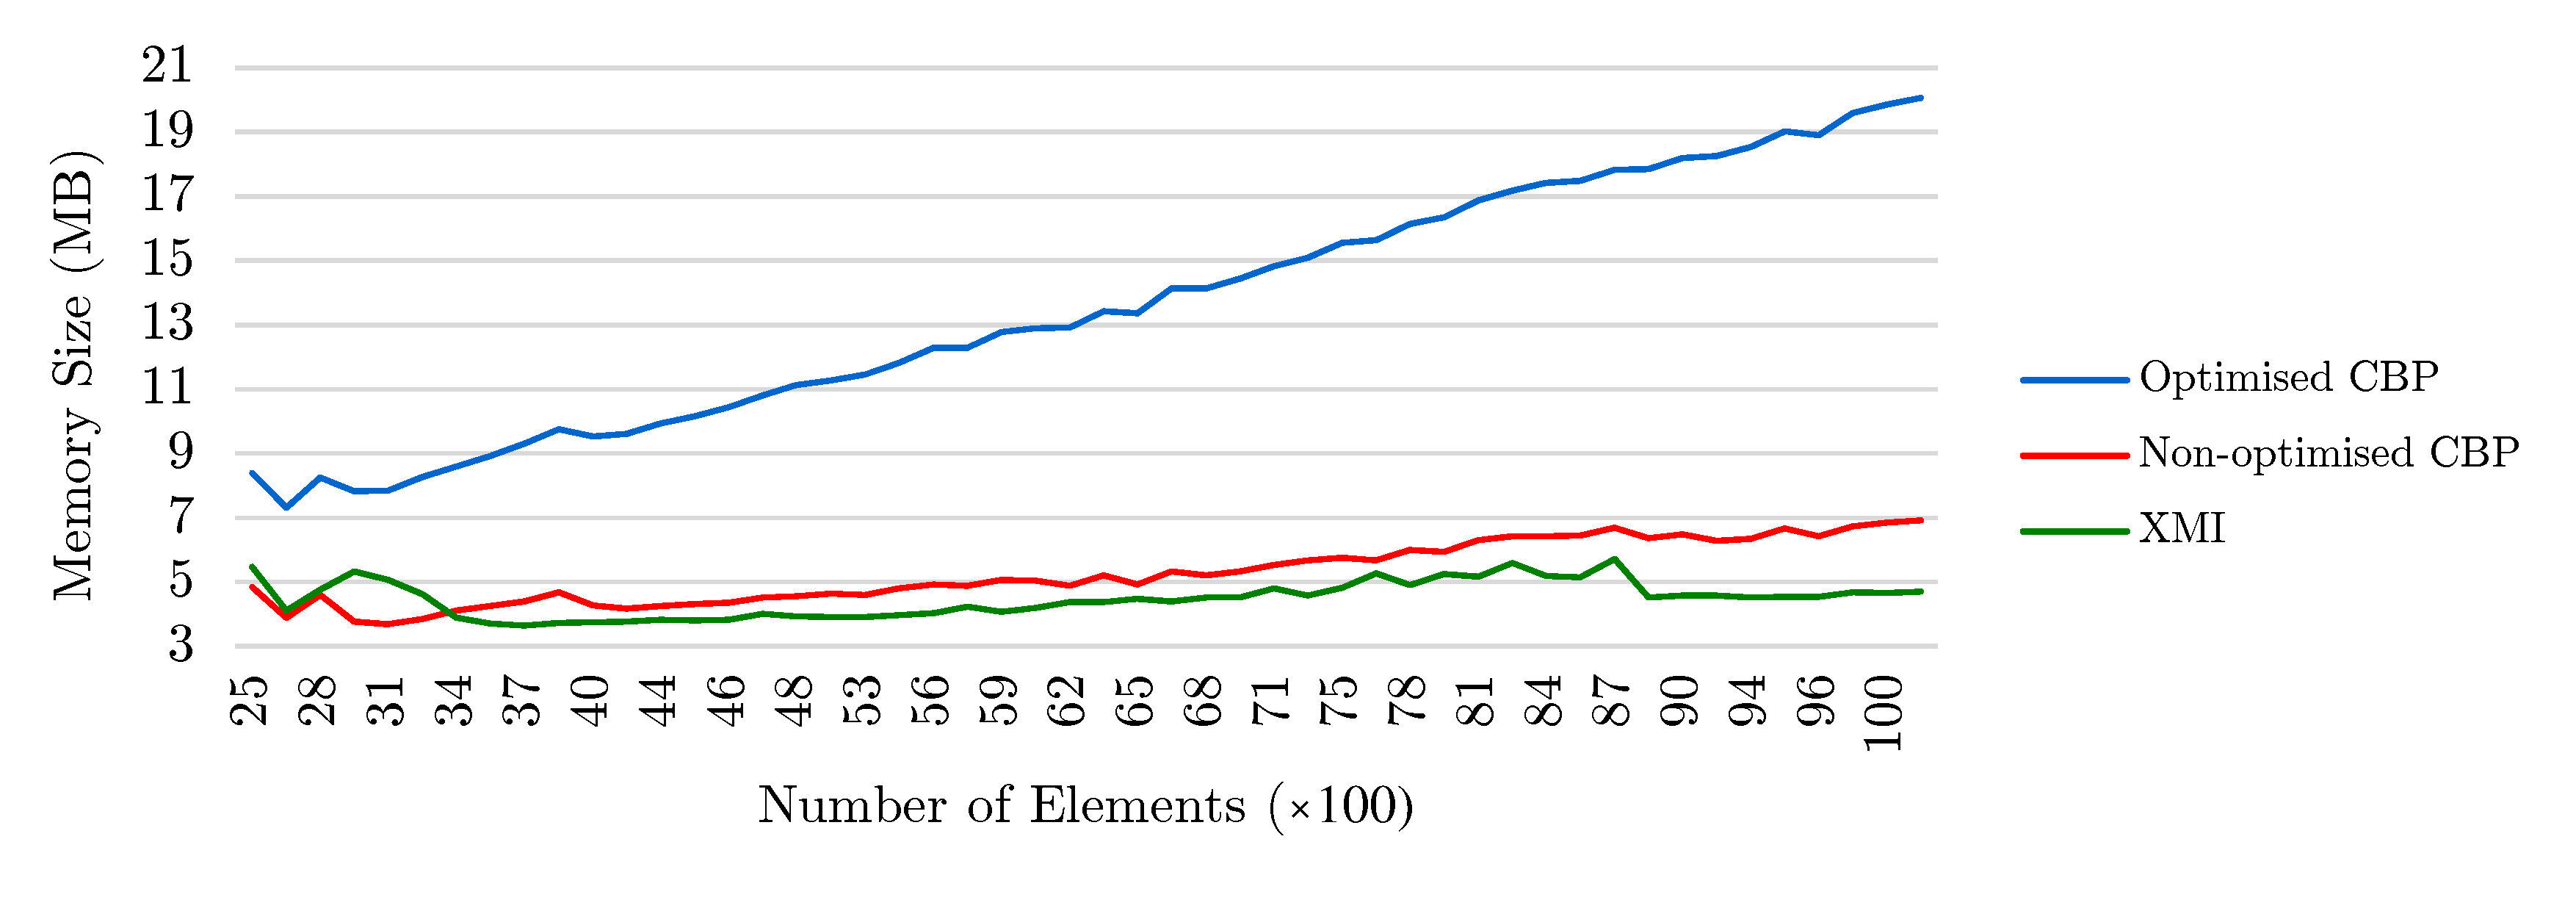
\includegraphics[width=\linewidth]{memory_ocbp_cbp_xmi}
	\caption{A comparison on memory footprints between optimised CBP, non-optimised CBP, and XMI after loading models.}\label{fig:memory_ocbp_cbp_xmi}
\end{figure}

\subsubsection{Threats to Validity and Limitations}
\label{sec:limitations_and_future_work}
In this work, this work has only tested the algorithm on synthesised conference models which may not be representative of the complexity and interconnectedness of models in other domains. Diverse characteristics of models in different domains can affect the effectiveness of the algorithm and therefore yield different outcomes. 

This work only supports ordered and unique features so far. Support for duplicate values means that removal of an item does not necessarily result in the item not being present in the feature value. Additional information must be captured to persist the number of copies and positions of the feature members. In the algorithms, this information can be used to properly generate the ignore list. In the case of unordered features, ``moved'' events do not exist, and hence further analysis is required to determine how this affects the use of the \emph{featureIsMoved} flag. 

\bibliographystyle{IEEEtran}
\bibliography{references}




%\begin{appendices}
%\end{appendices}

\end{document}